% Options for packages loaded elsewhere
\PassOptionsToPackage{unicode}{hyperref}
\PassOptionsToPackage{hyphens}{url}
\documentclass[
]{article}
\usepackage{xcolor}
\usepackage[a4paper,margin=1in]{geometry}
\usepackage{amsmath,amssymb}
\setcounter{secnumdepth}{-\maxdimen} % remove section numbering
\usepackage{iftex}
\ifPDFTeX
  \usepackage[T1]{fontenc}
  \usepackage[utf8]{inputenc}
  \usepackage{textcomp} % provide euro and other symbols
\else % if luatex or xetex
  \usepackage{unicode-math} % this also loads fontspec
  \defaultfontfeatures{Scale=MatchLowercase}
  \defaultfontfeatures[\rmfamily]{Ligatures=TeX,Scale=1}
\fi
\usepackage{lmodern}
\ifPDFTeX\else
  % xetex/luatex font selection
  \setmainfont[]{Times New Roman}
  \setsansfont[]{Arial}
  \setmonofont[]{Menlo}
\fi
% Use upquote if available, for straight quotes in verbatim environments
\IfFileExists{upquote.sty}{\usepackage{upquote}}{}
\IfFileExists{microtype.sty}{% use microtype if available
  \usepackage[]{microtype}
  \UseMicrotypeSet[protrusion]{basicmath} % disable protrusion for tt fonts
}{}
\usepackage{setspace}
\makeatletter
\@ifundefined{KOMAClassName}{% if non-KOMA class
  \IfFileExists{parskip.sty}{%
    \usepackage{parskip}
  }{% else
    \setlength{\parindent}{0pt}
    \setlength{\parskip}{6pt plus 2pt minus 1pt}}
}{% if KOMA class
  \KOMAoptions{parskip=half}}
\makeatother
\usepackage{longtable,booktabs,array}
\newcounter{none} % for unnumbered tables
\usepackage{calc} % for calculating minipage widths
% Correct order of tables after \paragraph or \subparagraph
\usepackage{etoolbox}
\makeatletter
\patchcmd\longtable{\par}{\if@noskipsec\mbox{}\fi\par}{}{}
\makeatother
% Allow footnotes in longtable head/foot
\IfFileExists{footnotehyper.sty}{\usepackage{footnotehyper}}{\usepackage{footnote}}
\makesavenoteenv{longtable}
\setlength{\emergencystretch}{3em} % prevent overfull lines
\providecommand{\tightlist}{%
  \setlength{\itemsep}{0pt}\setlength{\parskip}{0pt}}
\usepackage{etoolbox}
\usepackage{caption}
\usepackage{fvextra}

\preto\section{\clearpage}

% Keep captions tighter even when body text uses 1.5 spacing
\captionsetup{font={stretch=1}}

% Pandoc code blocks
\RecustomVerbatimEnvironment{Highlighting}{Verbatim}{
  commandchars=\\\{\},
  breaklines=true,
  breakanywhere=true,
  fontsize=\small,
  frame=single,
  framerule=0.3pt,
  framesep=2mm
}
\usepackage{bookmark}
\IfFileExists{xurl.sty}{\usepackage{xurl}}{} % add URL line breaks if available
\urlstyle{same}
\hypersetup{
  hidelinks,
  pdfcreator={LaTeX via pandoc}}

\author{}
\date{}

\begin{document}

\begin{titlepage}
\centering
\vspace*{\fill}

{\Huge \textbf{COMP4801 Final Year Project Report}\par}
\vspace{1cm}
{\LARGE Exploring Optimization Opportunity for WhatsHap\par}

\vspace{2cm}

{\large
Ng Ching Lap\par
UID: 3035687742\par
Supervisor: Professor Luo, Ruibang\par
}

\vspace*{\fill}
\end{titlepage}

\pagenumbering{roman}
\setcounter{page}{1}
\tableofcontents
\clearpage

\setstretch{1.5}
\section{Abstract}\label{abstract}

Haplotype phasing assigns heterozygous variants to their chromosome of
origin and is a key step in genomic analysis. Long-read sequencing
technologies (e.g., Oxford Nanopore Technologies, ONT) provide reads
spanning many variants and can improve phasing contiguity. However,
practical phasing performance depends on upstream alignment and variant
calling, and on long-read characteristics such as non-uniform coverage,
repetitive regions, and structured error patterns. WhatsHap is a widely
used phasing tool for long reads; systematically understanding its
end-to-end behavior under realistic conditions requires a controlled and
reproducible benchmarking environment.

This project builds a reproducible benchmarking pipeline that generates
a synthetic diploid reference genome, phased ground-truth variants and
haplotypes, simulates ONT-like reads with configurable realism knobs,
aligns reads, calls variants, phases using a vendored WhatsHap core, and
evaluates outputs against truth. The pipeline supports both oracle and
called variant sets to separate phaser-limited and caller-limited
regimes. The implementation is validated with unit tests and an
end-to-end test run, and the framework is then used for ablations and
parameter sweeps to isolate failure modes and identify optimization
directions for practical WhatsHap usage and long-read phasing workflows.

\clearpage
\pagenumbering{arabic}
\setcounter{page}{1}

\section{1. Introduction}\label{introduction}

Haplotype phasing assigns heterozygous variants to their chromosome of
origin, enabling downstream analyses such as compound heterozygosity
detection, allele-specific expression, and improved variant
interpretation. Long-read sequencing provides reads that span multiple
variants and can therefore improve both the contiguity and correctness
of phased haplotypes compared to short-read data. In practice, however,
phasing quality is not determined by the phasing algorithm alone: it is
affected by read alignment quality, variant calling accuracy, and
sequencing characteristics such as coverage bias, repetitive/duplicated
regions, and structured error patterns.

WhatsHap is one of the most widely adopted phasing tools for long reads.
While its algorithmic foundations are well studied, its behavior in
practical end-to-end pipelines can vary significantly depending on
upstream errors and data realism. A controlled benchmarking
environment---where individual factors can be varied independently and
runs can be reproduced reliably---is necessary to understand WhatsHap's
capabilities and limitations in realistic settings, and to identify
opportunities for optimization.

\subsection{1.1 Project goal}\label{project-goal}

This project aims to:

\begin{enumerate}
\def\labelenumi{\arabic{enumi}.}
\tightlist
\item
  Build a reproducible end-to-end benchmarking platform that mimics key
  characteristics of ONT-like long-read phasing workflows.
\item
  Evaluate WhatsHap's phasing capability under increasingly realistic
  conditions and quantify how different factors degrade performance.
\item
  Identify optimization directions or configuration recommendations for
  practical WhatsHap usage.
\end{enumerate}

\subsection{1.2 Contributions}\label{contributions}

\begin{itemize}
\tightlist
\item
  An end-to-end long-read simulation and benchmarking pipeline producing
  reference, truth variants/haplotypes, reads, alignments, variants,
  phased outputs, and standardized JSON/CSV reports.
\item
  A dual evaluation approach using \textbf{oracle} (ground-truth) and
  \textbf{called} variant sets to separate phasing limitations from
  variant-calling limitations.
\item
  Implemented realism ``knobs'' (e.g., duplicated regions, dropout,
  correlated error bursts, indel-rich truth) to isolate impacts on
  alignment/calling/phasing.
\item
  Automated experiment running, aggregation, and plotting to support
  systematic studies and report-ready results.
\end{itemize}

\subsection{1.3 Report organization}\label{report-organization}

Section 2 introduces background on long-read phasing, WhatsHap, and
evaluation metrics. Sections 3--9 describe requirements, design,
implementation, validation, configuration management, quality assurance,
and project management. Section 10 presents experimental results and
optimization investigations, followed by discussion and conclusions.

\section{2. Background}\label{background}

\subsection{2.1 Long-read sequencing and ONT-like
characteristics}\label{long-read-sequencing-and-ont-like-characteristics}

Long-read sequencing reads can span kilobases to megabases, often
covering many heterozygous variants within a single read. This enables
long-range phasing and reduces ambiguity compared to short reads. ONT
data, however, exhibits properties that complicate downstream analysis,
including higher raw error rates than short reads, a mixture of
substitution and indel errors, potential error clustering (bursts), and
non-uniform coverage due to sequencing and mapping biases. Repetitive
and duplicated regions further introduce ambiguity in read mapping,
which can degrade both variant calling and phasing.

\subsection{2.2 WhatsHap in practical pipelines (VCF + BAM → phased
VCF)}\label{whatshap-in-practical-pipelines-vcf-bam-phased-vcf}

In a typical long-read workflow, reads are aligned to a reference to
produce BAM/CRAM, variants are called to produce a VCF containing
genotypes, and a phasing tool assigns heterozygous variants to
haplotypes. WhatsHap takes aligned reads (BAM) and variants (VCF) and
extracts read-backed allele observations at variant positions. It then
partitions heterozygous variants into phase blocks and computes a
phasing solution within each block under an error-correction objective.
The output is a phased VCF where heterozygous genotypes are phased
(\texttt{0\textbar{}1} / \texttt{1\textbar{}0}) and annotated with phase
set identifiers (\texttt{PS}) indicating blocks.

\subsection{2.3 Why end-to-end benchmarking is
necessary}\label{why-end-to-end-benchmarking-is-necessary}

Phasing performance depends on multiple stages:

\begin{itemize}
\tightlist
\item
  \textbf{Alignment:} mapping quality, ambiguous mappings in
  repeats/duplications, and alignment artifacts around indels.
\item
  \textbf{Variant calling:} missing true variants (recall loss),
  spurious variants (precision loss), and genotype errors.
\item
  \textbf{Phasing:} block fragmentation and phase inconsistencies
  (switch errors) among phased variants.
\end{itemize}

To understand where failures originate, this project evaluates WhatsHap
under two regimes:

\begin{itemize}
\tightlist
\item
  \textbf{Oracle VCF:} uses ground-truth variants to isolate phasing
  behavior given a correct variant set.
\item
  \textbf{Called VCF:} uses variants produced by a caller to measure
  realistic end-to-end performance, including caller limitations.
\end{itemize}

This separation makes it possible to distinguish ``phaser-limited''
regimes (phasing errors dominate) from ``caller-limited'' regimes
(missing/incorrect variants dominate).

\subsection{2.4 Metrics}\label{metrics}

This project reports metrics designed for long-read phasing:

\begin{itemize}
\tightlist
\item
  \textbf{Number of phase sets:} a measure of block fragmentation
  (fewer/larger blocks generally indicate better long-range phasing).
\item
  \textbf{Switch error rate:} the fraction of adjacent phased
  heterozygous variants where predicted phase flips relative to truth.
\item
  \textbf{Phasing rate on shared heterozygous sites:} the fraction of
  shared heterozygous variants that are phased.
\item
  \textbf{Effective phased recall:} an end-to-end metric combining
  variant set overlap and correctness of phasing on truth heterozygous
  variants (used to compare oracle vs called regimes consistently).
\end{itemize}

\section{10. Experimental Evaluation}\label{experimental-evaluation}

\subsection{10.1 Experimental methodology and common
setup}\label{experimental-methodology-and-common-setup}

\subsubsection{10.1.1 Environment and
toolchain}\label{environment-and-toolchain}

\begin{itemize}
\tightlist
\item
  OS / CPU: macOS / Apple M2 Max
\item
  Python version: 3.12.12
\item
  minimap2 version: 2.30-r1287
\item
  samtools version: 1.23
\item
  bcftools version: 1.23
\item
  Vendored WhatsHap core path:
  \texttt{vendor/whatshap\_core/whatshap/core.\textless{}platform-specific\ extension\textgreater{}}
\end{itemize}

\subsubsection{10.1.2 Pipeline regimes}\label{pipeline-regimes}

\begin{itemize}
\tightlist
\item
  \textbf{Oracle regime:} phase using \texttt{*.oracle.vcf.gz}
  (phaser-limited)
\item
  \textbf{Called regime:} phase using \texttt{*.called.vcf.gz}
  (end-to-end)
\item
  \textbf{Indel policy:} when indels are enabled, use SNP-only
  phasing/evaluation (\texttt{phase\_snps\_only},
  \texttt{eval\_snps\_only})
\end{itemize}

For this project, a custom adaptor layer was used to construct the
\texttt{ReadSet} consumed by the vendored WhatsHap core. This was
necessary to support the study's experimental requirements, including
oracle vs called benchmarking, unified JSON provenance, and controlled
SNP-only phasing/evaluation under indel-containing truth sets. The
adaptor is therefore part of the project's benchmarking infrastructure
rather than a direct reproduction of the standard production-facing
WhatsHap front-end.

\subsubsection{10.1.3 Fixed parameters (baseline
constants)}\label{fixed-parameters-baseline-constants}

Unless stated otherwise in a subsection, experiments use the baseline
defaults defined by the experiment driver. These parameters control each
stage of the end-to-end pipeline (reference/truth generation → read
simulation → alignment → calling → phasing → evaluation).

\textbf{Reference generation} - \textbf{\texttt{ref\_length}}: Length of
the synthetic reference genome (bp). Larger references reduce boundary
effects and allow realism stressors (e.g., duplications) to be placed
without overlap. - \textbf{\texttt{ref\_preset}}: Reference ``complexity
preset'' (e.g., \texttt{plain} vs \texttt{realistic}). Presets control
the presence of hard regions (e.g., repetitive or biased regions) and
are recorded in \texttt{*.ref.meta.json}. -
\textbf{\texttt{dup\_segments}}: Number of duplicated segments
introduced into the reference. Higher values create more ambiguous
mapping, typically reducing calling recall and increasing phasing
fragmentation. - \textbf{\texttt{dup\_len}}: Length (bp) of each
duplicated segment copied from one locus to another. -
\textbf{\texttt{dup\_min\_gap}}: Minimum separation (bp) enforced
between duplicated segments/placements to avoid trivial overlaps.

\textbf{Truth generation} - \textbf{\texttt{num\_snps}}: Number of SNP
sites inserted into the truth set. Controls variant density and the
potential number of heterozygous loci for phasing. -
\textbf{\texttt{het\_rate}}: Fraction of truth SNPs that are
heterozygous (e.g., 0/1). WhatsHap only needs to phase heterozygous
sites; homozygous sites do not contribute phasing difficulty. -
\textbf{\texttt{phased\_truth}}: Whether the truth VCF contains phased
GT (e.g., \texttt{0\textbar{}1}). This is required for
switch-error-based evaluation. - \textbf{\texttt{random\_phase}}:
Whether truth phase orientation is randomly assigned per site (used to
avoid biasing truth haplotypes). - \textbf{Indel parameters (only when
enabled)}: - \textbf{\texttt{num\_indels}}: Number of indel variants
introduced into truth. - \textbf{\texttt{indel\_min\_len},
\texttt{indel\_max\_len}}: Indel length range (bp). Larger indels can
increase representation differences between truth/called sets. -
\textbf{\texttt{indel\_het\_rate}}: Fraction of indels that are
heterozygous.

\textbf{Read simulation} - \textbf{\texttt{platform}}: Read simulation
platform (e.g., \texttt{ont}). Determines error profile assumptions. -
\textbf{\texttt{ont\_profile}}: Preset for
substitution/insertion/deletion rates and base-quality characteristics
(e.g., \texttt{q20}). Used to approximate practical ONT error rates. -
\textbf{\texttt{num\_reads}}: Number of reads simulated. This acts as a
proxy for sequencing depth in this synthetic setting. -
\textbf{\texttt{min\_len}, \texttt{max\_len}}: Bounds on read lengths
(bp). Affects overlap connectivity (and therefore phasing block sizes).
- \textbf{\texttt{hap1\_frac}}: Fraction of reads sampled from haplotype
1 (vs haplotype 2). Typically 0.5 for balanced coverage. -
\textbf{Length model parameters}: - \textbf{\texttt{len\_model}}:
Distribution used to draw read lengths (e.g., \texttt{uniform} or
\texttt{lognormal}). - \textbf{\texttt{ln\_mean}, \texttt{ln\_sigma}}:
Parameters of the lognormal model (used when
\texttt{len\_model=lognormal}). - \textbf{Start/coverage model
parameters}: - \textbf{\texttt{start\_model}}: How read start positions
are sampled (e.g., \texttt{uniform} vs \texttt{dropout}). -
\textbf{\texttt{dropout\_fraction}}: Fraction of the reference affected
by coverage dropout (low/near-zero coverage windows). -
\textbf{\texttt{dropout\_block\_len}}: Typical length of dropout blocks
(bp), controlling the size of connectivity gaps. - \textbf{Correlated
error burst parameters}: - \textbf{\texttt{burst\_prob}}: Probability a
read contains one or more ``bursts'' of elevated error. -
\textbf{\texttt{burst\_count}}: Number of bursts injected into a read
(often fixed or bounded). - \textbf{\texttt{burst\_len}}: Length of each
burst (bp). - \textbf{\texttt{burst\_mult}}: Multiplier applied to base
error rates within bursts (higher → more severe).

\textbf{Alignment and calling thresholds} -
\textbf{\texttt{map\_preset}}: Minimap2 mapping preset (e.g.,
\texttt{map-ont}). Chosen to match ONT alignment behavior. -
\textbf{\texttt{call\_min\_mapq}}: Minimum mapping quality for reads to
be included in variant calling (\texttt{bcftools\ mpileup\ -q}). Higher
thresholds reduce ambiguous mappings but may reduce coverage. -
\textbf{\texttt{call\_min\_baseq}}: Minimum base quality for bases to
contribute to variant calling (\texttt{bcftools\ mpileup\ -Q}). Higher
thresholds reduce noisy evidence but may reduce sensitivity.

\textbf{Phasing parameters (WhatsHap integration)} -
\textbf{\texttt{vcf\_source}}: Which VCF to use for phasing: -
\texttt{oracle}: truth-derived variant set (isolates phasing), -
\texttt{called}: called variant set (end-to-end), - \texttt{both}: run
both for attribution. - \textbf{\texttt{max\_coverage}}: WhatsHap
read-selection cap (maximum effective coverage retained). Larger values
retain more reads (potentially better connectivity) but increase
compute. - \textbf{\texttt{min\_mapq}}: Minimum mapping quality for
reads to be used in phasing (driver filter). Controls how aggressively
ambiguous alignments are excluded. - \textbf{\texttt{min\_baseq}}:
Minimum base quality for allele observations used in phasing (driver
filter). Controls how aggressively noisy allele calls are excluded. -
\textbf{Indel-safe evaluation policy flags}: -
\textbf{\texttt{phase\_snps\_only}}: Filter \emph{input to phasing} to
biallelic SNPs only. - \textbf{\texttt{eval\_snps\_only}}: Filter
\emph{truth used for evaluation} to biallelic SNPs only. These flags
prevent indel representation differences from corrupting SNP phasing
evaluation.

\subsubsection{\texorpdfstring{10.1.4 Metrics reported (from
\texttt{aggregate.csv})}{10.1.4 Metrics reported (from aggregate.csv)}}\label{metrics-reported-from-aggregate.csv}

Metrics are computed per run from \texttt{*.pipeline.json} and
\texttt{*.eval.json}, then aggregated across seeds into
\texttt{aggregate.csv}. We report both \textbf{oracle} (phaser-focused)
and \textbf{called} (end-to-end) metrics to attribute performance loss
to variant calling vs phasing.

\textbf{Calling quality (called regime only)} -
\textbf{\texttt{call\_precision}}: Fraction of called SNPs that match
truth SNP sites (low precision indicates false positives).\\
Intuition: ``How many called variants are correct?'' -
\textbf{\texttt{call\_recall}}: Fraction of truth SNPs recovered by the
caller (low recall indicates missed variants).\\
Intuition: ``How many true variants were found?'' -
\textbf{\texttt{truth\_snps}}: Number of SNP records in the truth set
(after any SNP-only filtering). - \textbf{\texttt{called\_snps}}: Number
of SNP records produced by the caller. - \textbf{\texttt{shared\_snps}}:
Number of SNP records present in both truth and called sets (the overlap
the phaser can actually work with in called regime).

\textbf{Phasing coverage / completeness} -
\textbf{\texttt{*\_shared\_het\_recall}} (called): Fraction of truth
heterozygous SNPs that appear in the phasing input overlap (i.e., how
many true hets survive calling and exact matching).\\
This captures the ``caller bottleneck'' for phasing. -
\textbf{\texttt{*\_phasing\_rate\_shared\_het}} (called): Fraction of
shared heterozygous SNPs that end up phased (i.e., GT becomes
\texttt{0\textbar{}1} or \texttt{1\textbar{}0}).\\
This captures the ``phaser completeness'' \emph{given} available het
sites. - \textbf{\texttt{*\_effective\_phased\_recall}} (oracle/called):
Fraction of truth heterozygous SNPs that are both (a) present in the
evaluation set and (b) phased correctly (under best block flip).\\
This is the main ``end-to-end usable phasing'' metric.

\textbf{Phasing correctness} - \textbf{\texttt{*\_phase\_accuracy}}
(oracle/called): Accuracy of phased heterozygous genotypes under an
optimal global flip per phase set.\\
Reason: haplotypes are label-symmetric (swap hap1/hap2 yields equivalent
solution), so evaluation must be flip-invariant. -
\textbf{\texttt{*\_switch\_error}} (oracle/called): Switch error rate,
computed as \texttt{\#switches\ /\ \#adjacent\_het\_pairs\_compared}.\\
Interpretation: how often the predicted phase relationship between
adjacent heterozygous variants is inconsistent with truth.\\
Switch error is often the most informative correctness metric in
long-read phasing.

\textbf{Phase block fragmentation} -
\textbf{\texttt{*\_num\_phase\_sets}} (oracle/called): Number of
distinct phase sets (\texttt{PS}) in the phased VCF.\\
Lower is better (fewer blocks means longer haplotype continuity), but
extremely low values can also occur if very few het sites are phased. -
\textbf{Phase set size distribution (from eval JSON)}: Per-phase-set
sizes and best-flip matches.\\
Used to interpret whether fragmentation is driven by coverage gaps
(dropout), ambiguous mapping (duplications), or filtering thresholds.

\textbf{Runtime / efficiency} - \textbf{\texttt{time\_total\_sec}}:
Total pipeline runtime per run (if recorded).\\
Used in optimization sweeps to quantify trade-offs between
accuracy/continuity and compute.

\textbf{Oracle vs called interpretation} - Oracle metrics represent
``phaser-limited'' performance (variants are correct). - Called metrics
represent ``end-to-end'' performance (caller + phaser). - The gap
between oracle and called effective phased recall indicates how much
performance is lost due to variant calling overlap rather than phasing
itself.

\begin{center}\rule{0.5\linewidth}{0.5pt}\end{center}

\subsection{10.2 Baseline: depth scaling (coverage proxy via
num\_reads)}\label{baseline-depth-scaling-coverage-proxy-via-num_reads}

\subsubsection{Aim}\label{aim}

Establish baseline performance curves as sequencing depth increases, and
attribute performance limitations by comparing the oracle
(phaser-limited) regime against the called (end-to-end) regime.

\subsubsection{Setup}\label{setup}

\begin{itemize}
\tightlist
\item
  Varied: \texttt{num\_reads\ ∈\ \{50,\ 100,\ 200,\ 400\}} (3 seeds
  each)
\item
  Fixed: ONT-like simulation profile (q20), reference length 80 kb, 800
  truth SNPs (het rate 0.8), read length range 2--6 kb, calling
  thresholds (mapQ/baseQ), and phasing thresholds (max\_coverage,
  min\_mapq, min\_baseq) as specified in §10.1.
\end{itemize}

\subsubsection{Figures to include}\label{figures-to-include}

\begin{itemize}
\tightlist
\item
  \textbf{Figure 10.2.1 --- Variant calling recall vs sequencing depth.}
\item
  \textbf{Figure 10.2.2 --- Oracle effective phased recall vs sequencing
  depth (phasing-only upper bound).}
\item
  \textbf{Figure 10.2.3 --- Called effective phased recall vs sequencing
  depth (end-to-end performance).}
\item
  \textbf{Figure 10.2.4 --- Oracle number of phase sets vs sequencing
  depth (block fragmentation, phasing-only).}
\item
  \textbf{Figure 10.2.5 --- Called number of phase sets vs sequencing
  depth (block fragmentation, end-to-end).}
\item
  \textbf{Figure 10.2.6 --- Called switch error rate vs sequencing
  depth.}
\end{itemize}

\textbf{Figure 10.2.1 --- Variant calling recall vs sequencing depth.}\\
Calling recall is computed as \texttt{shared\_snps\ /\ truth\_snps},
where \texttt{shared\_snps} are SNP records present in both the truth
VCF and the called VCF (exact-position matching in the pipeline's
callset summary). As read depth increases (num\_reads), recall increases
sharply, indicating that \emph{variant discovery} is the main limiter at
low coverage. Points show mean over seeds; error bars show standard
deviation.

\textbf{Figure 10.2.2 --- Oracle effective phased recall vs sequencing
depth (phasing-only upper bound).}\\
Oracle effective phased recall measures WhatsHap's phasing performance
when the input variants are ``oracle'' (truth-derived SNP sites),
removing variant calling errors from the pipeline. The curve rises with
depth and approaches a high plateau, representing the phasing-only
capability under the simulated ONT Q20 error model. Points show mean
over seeds; error bars show standard deviation.

\begin{center}
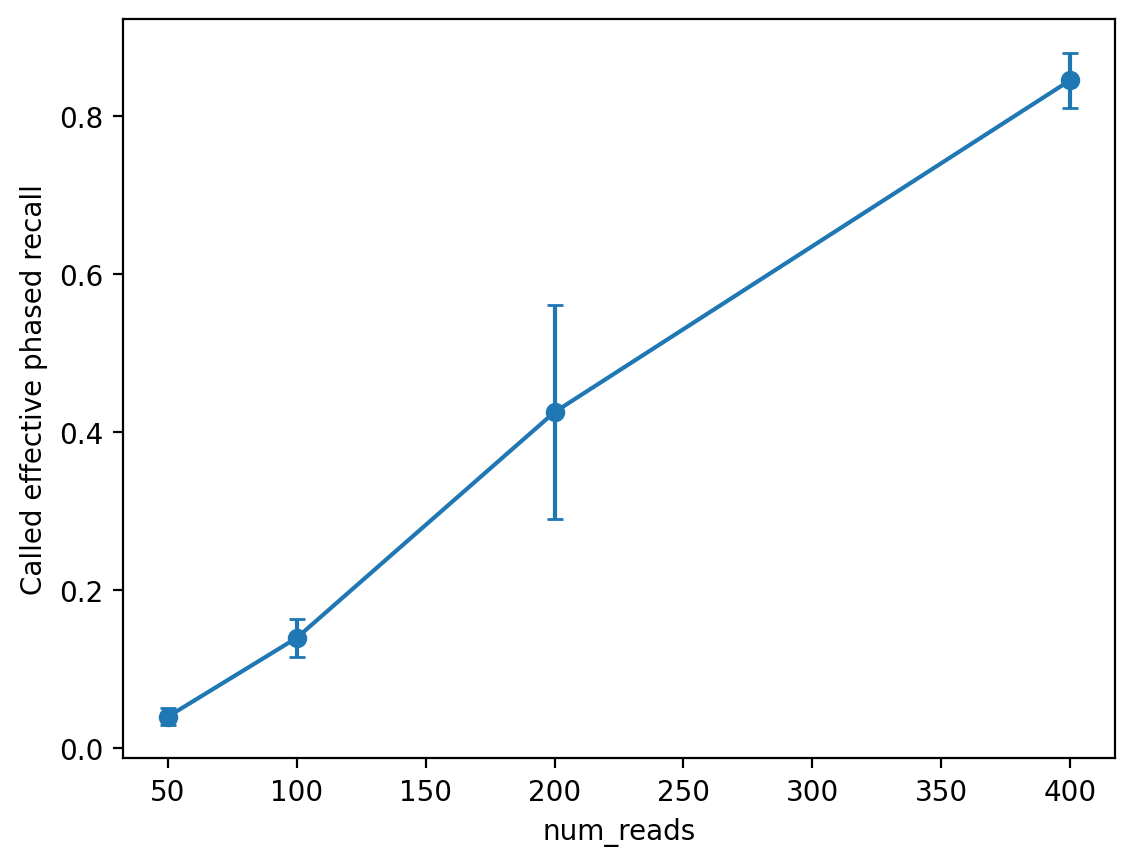
\includegraphics[width=0.82\linewidth]{figures/10_experiments/fig_10_2_3_called_effective_phased_recall.png}
\end{center}

\textbf{Figure 10.2.3 --- Called effective phased recall vs sequencing
depth (end-to-end performance).} Called effective phased recall measures
the fraction of truth heterozygous SNPs that end up \emph{both present
in the called set and correctly phased} (after best block flip). This
curve is substantially lower than the oracle curve at low depth,
demonstrating that variant calling recall (and callset composition)
dominates end-to-end phasing performance early on. Points show mean over
seeds; error bars show standard deviation.

\textbf{Figure 10.2.4 --- Oracle number of phase sets vs sequencing
depth (block fragmentation, phasing-only).}\\
The number of phase sets (PS blocks) reflects \emph{fragmentation}: more
phase sets means shorter blocks / less connectivity. Under oracle
variants, increasing depth reduces fragmentation as reads bridge more
heterozygous sites. Points show mean over seeds; error bars show
standard deviation.

\textbf{Figure 10.2.5 --- Called number of phase sets vs sequencing
depth (block fragmentation, end-to-end).}\\
The phase-set count using called variants reflects fragmentation under
end-to-end conditions. Unlike the oracle curve, this may be
non-monotonic at moderate depths because the called VCF changes with
depth (different sites called and filtered), affecting graph
connectivity. Points show mean over seeds; error bars show standard
deviation.

\textbf{Figure 10.2.6 --- Called switch error rate vs sequencing
depth.}\\
Switch error rate is computed over adjacent phased heterozygous SNP
pairs within phase sets (after choosing the best global flip per phase
set). The mean generally decreases as depth increases, but can show
variance at intermediate depths due to small denominators and changing
callsets. Error bars show standard deviation; interpret values as
bounded to {[}0, 1{]} even if \texttt{mean\ ±\ std} extends below 0.

\subsubsection{Results summary (means over
seeds)}\label{results-summary-means-over-seeds}

Calling (called regime): - \texttt{call\_recall}: 0.224 (50) → 0.399
(100) → 0.662 (200) → 0.877 (400) - \texttt{call\_precision}: 1.000 at
all depths in this synthetic setup (no SNP false positives observed)

Oracle phasing (phaser-limited): -
\texttt{oracle\_effective\_phased\_recall}: 0.513 → 0.750 → 0.921 →
0.969 - \texttt{oracle\_switch\_error}: near 0 across all depths -
\texttt{oracle\_num\_phase\_sets}: 10.7 → 5.7 → 1.7 → 1.0

Called phasing (end-to-end): -
\texttt{called\_effective\_phased\_recall}: 0.040 → 0.140 → 0.426 →
0.845 - \texttt{called\_shared\_het\_recall}: 0.129 → 0.281 → 0.590 →
0.854 - \texttt{called\_phasing\_rate\_shared\_het}: 0.355 → 0.517 →
0.808 → 0.991 - \texttt{called\_switch\_error}: high variance at
100--200 reads (outlier seeds), near 0 at 400 reads -
\texttt{called\_num\_phase\_sets}: 5.0 → 7.7 → 3.0 → 1.0 (non-monotonic
due to changing number of phased het sites)

Taken together, these decomposition terms show that most loss in called
effective phased recall arises from reduced shared heterozygous site
recall rather than from poor phase accuracy, indicating that variant
recovery and connectivity are the dominant bottlenecks in the baseline
setting.

\subsubsection{Key observations}\label{key-observations}

\begin{itemize}
\tightlist
\item
  O1 (Calling is depth-limited): Calling recall increases strongly with
  \texttt{num\_reads} (0.224 → 0.877), indicating the caller is
  primarily sensitivity-limited at low/moderate depth. Precision remains
  1.0 in this controlled setup, so errors manifest mainly as missed
  sites rather than spurious sites.
\item
  O2 (WhatsHap is accurate given correct sites): In the oracle regime,
  switch error is \textasciitilde0 and phase accuracy is
  \textasciitilde1 even at low depth; the main limitation at 50--100
  reads is incompleteness (many het sites remain unphased due to
  connectivity gaps).
\item
  O3 (Residual high-depth loss remains caller-limited): At 400 reads,
  called phasing is nearly perfect on shared heterozygous sites (phasing
  rate ≈ 0.99, accuracy ≈ 1.0). The remaining gap between oracle and
  called effective phased recall is therefore dominated by missing
  heterozygous sites in the called set
  (\texttt{called\_shared\_het\_recall} ≈ 0.85).
\item
  O4 (Mid-depth instability in called regime): At 100--200 reads, the
  called regime shows occasional high switch error in individual seeds.
  This likely reflects both seed sensitivity and small denominators in
  switch-error calculation when the called VCF contains relatively few
  informative heterozygous sites. This motivates using more seeds in the
  final pass.
\end{itemize}

\subsubsection{Takeaway}\label{takeaway}

The baseline depth sweep confirms that the pipeline behaves sensibly:
calling recall increases with depth; oracle phasing becomes both
accurate and contiguous with increasing depth; and end-to-end (called)
phasing improves sharply but remains limited primarily by the overlap of
correctly called heterozygous variants. At sufficiently high depth (400
reads in this setup), WhatsHap phasing is essentially correct on
available het sites, implying that further end-to-end gains would
require improvements in variant calling overlap rather than the phasing
algorithm itself.

\begin{center}\rule{0.5\linewidth}{0.5pt}\end{center}

\subsection{10.3 Single-knob study: duplicated regions (reference
stressor)}\label{single-knob-study-duplicated-regions-reference-stressor}

\subsubsection{Aim}\label{aim-1}

Measure how duplicated reference segments affect end-to-end phasing by
increasing mapping ambiguity, and determine whether the main impact is
on variant recovery, phasing continuity, or phasing correctness.

\subsubsection{Setup}\label{setup-1}

\begin{itemize}
\tightlist
\item
  Varied: \texttt{dup\_segments\ ∈\ \{0,\ 1,\ 3,\ 5\}} (3 seeds each by
  default; 5 seeds recommended if runtime allows)
\item
  Fixed:

  \begin{itemize}
  \tightlist
  \item
    \texttt{dup\_len\ =\ 3000}
  \item
    \texttt{dup\_min\_gap\ =\ 500}
  \item
    baseline depth fixed at \texttt{num\_reads\ =\ 200}
  \item
    ONT-like simulation profile (\texttt{ont\_profile\ =\ q20})
  \item
    reference length \texttt{80\ kb}
  \item
    \texttt{800} truth SNPs (\texttt{het\_rate\ =\ 0.8})
  \item
    read length range \texttt{2–6\ kb}
  \item
    \texttt{start\_model\ =\ uniform}
  \item
    no dropout (\texttt{dropout\_fraction\ =\ 0.0})
  \item
    no correlated bursts (\texttt{burst\_prob\ =\ 0.0})
  \item
    no truth indels (\texttt{num\_indels\ =\ 0})
  \item
    phasing input source \texttt{vcf\_source\ =\ both}
  \end{itemize}
\end{itemize}

This experiment isolates duplicated sequence as a single realism
stressor while keeping all other baseline conditions unchanged.

\subsubsection{Figures to include}\label{figures-to-include-1}

\begin{itemize}
\tightlist
\item
  \textbf{Figure 10.3.1 --- Variant calling recall vs duplicated-region
  count.}
\item
  \textbf{Figure 10.3.2 --- Called effective phased recall vs
  duplicated-region count.}
\item
  \textbf{Figure 10.3.3 --- Called switch error rate vs
  duplicated-region count.}
\item
  \textbf{Figure 10.3.4 --- Oracle effective phased recall vs
  duplicated-region count.}
\item
  \textbf{Figure 10.3.5 --- Called number of phase sets vs
  duplicated-region count.}
\end{itemize}

\textbf{Figure 10.3.1 --- Variant calling recall vs duplicated-region
count.}\\
Calling recall remains nearly unchanged across duplication levels,
indicating that the duplicated-region stressor does not substantially
reduce SNP site recovery under the current alignment and calling
settings.

\textbf{Figure 10.3.2 --- Called effective phased recall vs
duplicated-region count.}\\
End-to-end phasing remains broadly stable at low-to-moderate duplication
levels, but declines at the highest duplication setting. This indicates
that duplicated regions only become a substantial stressor in the called
regime once ambiguity is sufficiently strong.

\textbf{Figure 10.3.3 --- Called switch error rate vs duplicated-region
count.}\\
Switch error remains modest at low-to-moderate duplication levels but
increases markedly at the highest duplication setting, suggesting that
duplicated regions can destabilize local phase relationships even when
overall call recall remains similar.

\textbf{Figure 10.3.4 --- Oracle effective phased recall vs
duplicated-region count.}\\
Oracle phasing performance remains high and stable across duplication
levels, showing that WhatsHap itself is robust when correct variant
sites are available and that the main duplication effect emerges in the
end-to-end called regime.

\textbf{Figure 10.3.5 --- Called number of phase sets vs
duplicated-region count.}\\
Phase-set count does not increase with duplication in this experiment
and therefore should not be interpreted in isolation. At the highest
duplication level, fewer phase sets coincide with worse phasing accuracy
and higher switch error, indicating that phase-set count alone is not a
sufficient measure of performance here.

\subsubsection{Results summary (means over
seeds)}\label{results-summary-means-over-seeds-1}

\begin{itemize}
\tightlist
\item
  \texttt{call\_recall}: 0.663 (0 dup) → 0.671 (1 dup) → 0.661 (3 dup) →
  0.666 (5 dup)
\item
  \texttt{call\_precision}: 1.000 at all duplication levels in this
  synthetic setup
\item
  \texttt{called\_effective\_phased\_recall}: 0.436 → 0.473 → 0.479 →
  0.372
\item
  \texttt{called\_shared\_het\_recall}: 0.590 → 0.599 → 0.586 → 0.593
\item
  \texttt{called\_phasing\_rate\_shared\_het}: 0.819 → 0.836 → 0.848 →
  0.778
\item
  \texttt{called\_phase\_accuracy}: 0.890 → 0.920 → 0.960 → 0.802
\item
  \texttt{called\_switch\_error}: 0.122 → 0.073 → 0.040 → 0.209
\item
  \texttt{called\_num\_phase\_sets}: 3.4 → 3.4 → 3.4 → 2.6
\item
  \texttt{oracle\_effective\_phased\_recall}: 0.925 → 0.932 → 0.924 →
  0.918
\item
  \texttt{oracle\_switch\_error}: near 0 across all duplication levels
\item
  \texttt{oracle\_num\_phase\_sets}: 1.8 → 1.8 → 1.2 → 1.8
\end{itemize}

Taken together, these results show that duplicated regions are a
relatively mild stressor under the current parameterization. The
strongest degradation appears only at the highest duplication level
(\texttt{dup\_segments\ =\ 5}), and is driven mainly by reduced
called-regime phasing completeness and phase accuracy rather than by
reduced callset overlap.

\subsubsection{Key observations}\label{key-observations-1}

\begin{itemize}
\item
  O1 (Calling recall is largely unaffected by duplication in this
  setup): Across \texttt{dup\_segments\ ∈\ \{0,1,3,5\}}, calling recall
  remains nearly flat (\texttt{0.663–0.671}) and call precision stays at
  1.0. This indicates that the current duplication stressor does not
  substantially reduce SNP site recovery under the baseline
  alignment/calling settings.
\item
  O2 (Oracle phasing remains stable): Oracle effective phased recall
  remains high and nearly unchanged (\texttt{0.918–0.932}), with
  near-zero oracle switch error throughout. This shows that when correct
  variant sites are supplied, WhatsHap itself remains robust to the
  duplicated-region stressor at these settings.
\item
  O3 (Called-regime degradation appears mainly at the highest
  duplication level): At \texttt{dup\_segments\ =\ 5}, called effective
  phased recall drops from \texttt{0.479} to \texttt{0.372}, while
  called switch error rises from \texttt{0.040} to \texttt{0.209}.
  However, \texttt{called\_shared\_het\_recall} remains approximately
  constant (\texttt{\textasciitilde{}0.59}), indicating that the
  degradation is not primarily due to loss of shared heterozygous sites.
\item
  O4 (Main loss is in phasing completeness/correctness on surviving
  sites): The highest-duplication condition reduces
  \texttt{called\_phasing\_rate\_shared\_het} (\texttt{0.848\ →\ 0.778})
  and \texttt{called\_phase\_accuracy} (\texttt{0.960\ →\ 0.802}). This
  suggests that duplicated regions mainly weaken the consistency of
  phasing evidence in the called regime rather than simply reducing
  callset overlap.
\item
  O5 (Phase-set count is not the main signal here):
  \texttt{called\_num\_phase\_sets} does not increase with duplication,
  and is actually lower at \texttt{dup\_segments\ =\ 5}. In this
  experiment, lower phase-set count does not imply better phasing,
  because it occurs alongside lower effective phased recall and higher
  switch error. This indicates that phase-set count should be
  interpreted together with completeness and correctness metrics rather
  than in isolation.
\end{itemize}

\subsubsection{Takeaway}\label{takeaway-1}

Under the current parameterization, duplicated regions are a relatively
mild stressor for variant recovery and for oracle phasing. Their main
impact appears only at the highest duplication level, where end-to-end
(called) phasing becomes less complete and less accurate despite largely
unchanged callset overlap. This suggests that duplicated regions
primarily affect the quality and stability of phasing evidence in the
called regime, rather than acting as a strong caller-limited bottleneck.
In other words, the duplication stressor in this setup is better
characterized as a called-regime phasing/evidence-quality stressor than
as a pure site-recovery stressor.

\begin{center}\rule{0.5\linewidth}{0.5pt}\end{center}

\subsection{10.4 Single-knob study: coverage dropout (read start
model)}\label{single-knob-study-coverage-dropout-read-start-model}

\subsubsection{Aim}\label{aim-2}

Evaluate how localized coverage dropout affects phase-block continuity
and effective phased recall, and determine whether the main impact is on
variant recovery, phasing completeness, or both.

\subsubsection{Setup}\label{setup-2}

\begin{itemize}
\tightlist
\item
  Varied: \texttt{dropout\_fraction\ ∈\ \{0.00,\ 0.05,\ 0.10,\ 0.20\}}
\item
  Fixed:

  \begin{itemize}
  \tightlist
  \item
    \texttt{dropout\_block\_len\ =\ 1000}
  \item
    baseline depth fixed at \texttt{num\_reads\ =\ 200}
  \item
    ONT-like simulation profile (\texttt{ont\_profile\ =\ q20})
  \item
    reference length \texttt{80\ kb}
  \item
    \texttt{800} truth SNPs (\texttt{het\_rate\ =\ 0.8})
  \item
    read length range \texttt{2–6\ kb}
  \item
    \texttt{start\_model\ =\ dropout}
  \item
    no duplications (\texttt{dup\_segments\ =\ 0})
  \item
    no correlated bursts (\texttt{burst\_prob\ =\ 0.0})
  \item
    no truth indels (\texttt{num\_indels\ =\ 0})
  \item
    phasing input source \texttt{vcf\_source\ =\ both}
  \end{itemize}
\end{itemize}

This experiment isolates coverage dropout as a single realism stressor
while keeping the remaining baseline conditions unchanged.

\subsubsection{Figures to include}\label{figures-to-include-2}

\begin{itemize}
\tightlist
\item
  \textbf{Figure 10.4.1 --- Oracle number of phase sets vs dropout
  fraction.}
\item
  \textbf{Figure 10.4.2 --- Called number of phase sets vs dropout
  fraction.}
\item
  \textbf{Figure 10.4.3 --- Oracle effective phased recall vs dropout
  fraction.}
\item
  \textbf{Figure 10.4.4 --- Called effective phased recall vs dropout
  fraction.}
\item
  \textbf{Figure 10.4.5 --- Variant calling recall vs dropout fraction.}
\end{itemize}

\textbf{Figure 10.4.1 --- Oracle number of phase sets vs dropout
fraction.} The number of oracle phase sets increases strongly with
dropout fraction, showing that localized coverage gaps fragment
haplotype blocks even when correct variant sites are supplied to the
phaser.

\textbf{Figure 10.4.2 --- Called number of phase sets vs dropout
fraction.} End-to-end phase fragmentation increases at low-to-moderate
dropout levels, but phase-set count alone becomes harder to interpret at
severe dropout because many heterozygous sites are no longer called or
phased.

\textbf{Figure 10.4.3 --- Oracle effective phased recall vs dropout
fraction.} Oracle effective phased recall decreases as dropout
increases, indicating that coverage gaps directly reduce phasing
completeness by breaking read connectivity between heterozygous sites.

\begin{center}
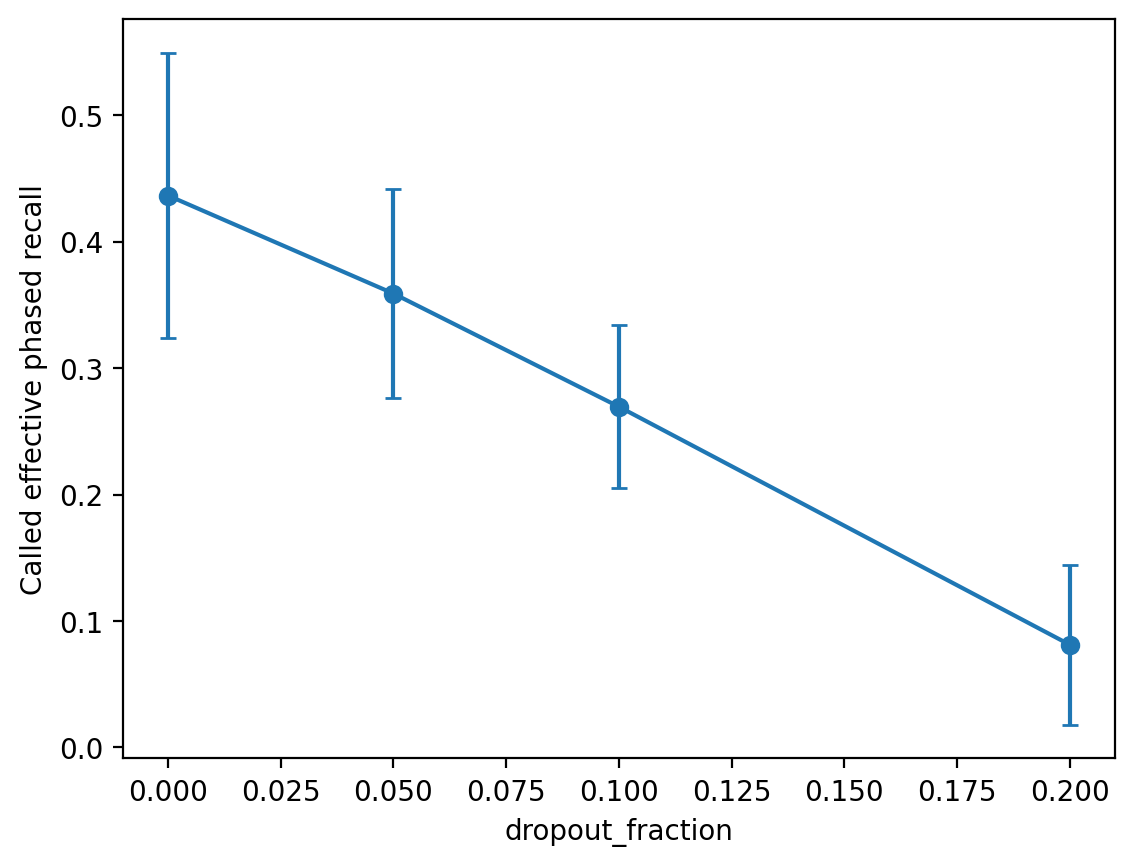
\includegraphics[width=0.82\linewidth]{figures/10_experiments/fig_10_4_4_called_effective_phased_recall.png}
\end{center}

\textbf{Figure 10.4.4 --- Called effective phased recall vs dropout
fraction.} Called effective phased recall declines much more steeply
than oracle effective phased recall, showing that dropout affects both
phasing connectivity and, at stronger dropout levels, variant recovery
in the called regime.

\textbf{Figure 10.4.5 --- Variant calling recall vs dropout fraction.}\\
Calling recall decreases gradually at moderate dropout and then sharply
at the strongest dropout level, indicating that severe low-coverage
regions substantially reduce the recovery of true SNP sites.

\subsubsection{Results summary (means over
seeds)}\label{results-summary-means-over-seeds-2}

\begin{itemize}
\tightlist
\item
  \texttt{call\_recall}: 0.663 (0.00) → 0.635 (0.05) → 0.605 (0.10) →
  0.432 (0.20)
\item
  \texttt{call\_precision}: 1.000 at all dropout levels in this
  synthetic setup
\item
  \texttt{oracle\_effective\_phased\_recall}: 0.925 → 0.865 → 0.857 →
  0.637
\item
  \texttt{oracle\_switch\_error}: near 0 across all dropout levels
\item
  \texttt{oracle\_num\_phase\_sets}: 1.8 → 2.8 → 3.2 → 10.0
\item
  \texttt{called\_effective\_phased\_recall}: 0.436 → 0.359 → 0.269 →
  0.081
\item
  \texttt{called\_shared\_het\_recall}: 0.590 → 0.565 → 0.529 → 0.362
\item
  \texttt{called\_phasing\_rate\_shared\_het}: 0.819 → 0.704 → 0.514 →
  0.239
\item
  \texttt{called\_phase\_accuracy}: 0.890 → 0.894 → 0.981 → 0.922
\item
  \texttt{called\_switch\_error}: 0.122 → 0.072 → 0.006 → 0.089
\item
  \texttt{called\_num\_phase\_sets}: 3.4 → 5.0 → 6.2 → 4.0
\end{itemize}

Decomposition of called effective phased recall shows that coverage
dropout first increases loss through unphased shared heterozygous sites
(fragmentation / reduced connectivity), and at the strongest dropout
level also causes a substantial increase in loss from missing called
sites.

\subsubsection{Key observations}\label{key-observations-2}

\begin{itemize}
\item
  O1 (Coverage dropout strongly increases fragmentation): In the oracle
  regime, the number of phase sets rises from \texttt{1.8} at
  \texttt{dropout\_fraction\ =\ 0.00} to \texttt{10.0} at \texttt{0.20},
  while oracle switch error remains near zero throughout. This shows
  that dropout primarily breaks phase-block continuity rather than
  causing incorrect phase assignments.
\item
  O2 (Dropout directly reduces phasing completeness even with correct
  variant sites): Oracle effective phased recall declines from
  \texttt{0.925} to \texttt{0.637} as dropout increases. Because oracle
  shared-site recall remains fixed by construction, this reduction is
  attributable to weaker read connectivity and more unphased
  heterozygous sites.
\item
  O3 (End-to-end performance degrades more strongly than oracle
  performance): Called effective phased recall falls from \texttt{0.436}
  to \texttt{0.081}, a steeper decline than in the oracle regime. This
  indicates that dropout harms end-to-end phasing through both
  connectivity loss and reduced overlap of correctly called heterozygous
  variants.
\item
  O4 (Moderate dropout is mainly a connectivity / completeness problem):
  From \texttt{dropout\_fraction\ =\ 0.00} to \texttt{0.10}, the main
  worsening in the called regime is a drop in
  \texttt{called\_phasing\_rate\_shared\_het} (\texttt{0.819\ →\ 0.514})
  together with increased fragmentation. This indicates that moderate
  dropout primarily prevents surviving heterozygous sites from being
  phased into long connected blocks.
\item
  O5 (Severe dropout becomes a mixed calling + phasing bottleneck): At
  \texttt{dropout\_fraction\ =\ 0.20}, \texttt{call\_recall} drops
  sharply to \texttt{0.432} and \texttt{called\_shared\_het\_recall}
  falls to \texttt{0.362}, while
  \texttt{called\_phasing\_rate\_shared\_het} also falls to
  \texttt{0.239}. This shows that strong dropout not only fragments
  phase blocks but also substantially reduces variant recovery in the
  called regime.
\item
  O6 (Switch error is not the main signal in this study): Although
  called switch error does not increase monotonically, this should not
  be interpreted as improved phasing at moderate dropout. As dropout
  increases, fewer heterozygous sites remain phased, making switch error
  less informative than completeness and fragmentation metrics.
\end{itemize}

\subsubsection{Takeaway}\label{takeaway-2}

Coverage dropout is a strong fragmentation-dominated stressor in this
pipeline. Its primary effect is to create low-coverage gaps that prevent
reads from connecting heterozygous sites into long phase blocks, which
reduces phasing completeness even in the oracle regime. In the called
regime, this effect is amplified, and at severe dropout levels the
stressor becomes mixed: both phase connectivity and variant recovery
deteriorate substantially. Overall, coverage dropout is one of the
clearest examples in this study of a realism knob that directly disrupts
haplotype continuity.

\begin{center}\rule{0.5\linewidth}{0.5pt}\end{center}

\subsection{10.5 Single-knob study: correlated error
bursts}\label{single-knob-study-correlated-error-bursts}

\subsubsection{Aim}\label{aim-3}

Assess how localized high-error segments within reads affect variant
calling and phasing stability, and determine whether the main impact is
on callset recovery, phasing correctness, or phasing completeness.

\subsubsection{Setup}\label{setup-3}

\begin{itemize}
\tightlist
\item
  Varied: \texttt{burst\_prob\ ∈\ \{0.0,\ 0.3,\ 0.6\}}
\item
  Fixed:

  \begin{itemize}
  \tightlist
  \item
    \texttt{burst\_count\ =\ 2}
  \item
    \texttt{burst\_len\ =\ 300}
  \item
    \texttt{burst\_mult\ =\ 8.0}
  \item
    baseline depth fixed at \texttt{num\_reads\ =\ 200}
  \item
    ONT-like simulation profile (\texttt{ont\_profile\ =\ q20})
  \item
    reference length \texttt{80\ kb}
  \item
    \texttt{800} truth SNPs (\texttt{het\_rate\ =\ 0.8})
  \item
    read length range \texttt{2–6\ kb}
  \item
    \texttt{start\_model\ =\ uniform}
  \item
    no duplications (\texttt{dup\_segments\ =\ 0})
  \item
    no coverage dropout (\texttt{dropout\_fraction\ =\ 0.0})
  \item
    no truth indels (\texttt{num\_indels\ =\ 0})
  \item
    phasing input source \texttt{vcf\_source\ =\ both}
  \end{itemize}
\end{itemize}

This experiment isolates correlated error bursts as a single realism
stressor while keeping the remaining baseline conditions unchanged.

\subsubsection{Figures to include}\label{figures-to-include-3}

\begin{itemize}
\tightlist
\item
  \textbf{Figure 10.5.1 --- Called switch error rate vs burst
  probability.}
\item
  \textbf{Figure 10.5.2 --- Called effective phased recall vs burst
  probability.}
\item
  \textbf{Figure 10.5.3 --- Variant calling recall vs burst
  probability.}
\item
  \textbf{Figure 10.5.4 --- Called number of phase sets vs burst
  probability.}
\item
  \textbf{Figure 10.5.5 --- Oracle effective phased recall vs burst
  probability.}
\end{itemize}

\textbf{Figure 10.5.1 --- Called switch error rate vs burst
probability.}\\
Called switch error shows a modest increase at the intermediate burst
setting, suggesting that correlated high-error segments can destabilize
local phase relationships in the end-to-end called regime. However, the
effect is not monotonic across the burst sweep.

\textbf{Figure 10.5.2 --- Called effective phased recall vs burst
probability.}\\
End-to-end phased recall decreases at \texttt{burst\_prob\ =\ 0.3} but
rebounds at \texttt{0.6}, indicating that the current burst stressor
produces a weak and somewhat noisy effect rather than a strong monotonic
degradation trend.

\textbf{Figure 10.5.3 --- Variant calling recall vs burst
probability.}\\
Calling recall remains broadly stable across burst settings, indicating
that correlated error bursts do not substantially reduce SNP site
recovery under the current parameterization.

\textbf{Figure 10.5.4 --- Called number of phase sets vs burst
probability.}\\
Phase-set count does not increase with burst probability and therefore
is not the main signal in this study. Under the current settings,
correlated error bursts appear to affect phasing correctness more than
fragmentation.

\textbf{Figure 10.5.5 --- Oracle effective phased recall vs burst
probability.}\\
Oracle phasing performance remains high and stable across burst
settings, showing that WhatsHap itself is robust when correct variant
sites are supplied and that the observed burst effect arises mainly in
the end-to-end called regime.

\subsubsection{Results summary (means over
seeds)}\label{results-summary-means-over-seeds-3}

\begin{itemize}
\tightlist
\item
  \texttt{call\_recall}: 0.663 (\texttt{burst\_prob\ =\ 0.0}) → 0.681
  (\texttt{0.3}) → 0.676 (\texttt{0.6})
\item
  \texttt{call\_precision}: 1.000 at all burst levels in this synthetic
  setup
\item
  \texttt{oracle\_effective\_phased\_recall}: 0.925 → 0.926 → 0.921
\item
  \texttt{oracle\_switch\_error}: near 0 across all burst levels
\item
  \texttt{oracle\_num\_phase\_sets}: 1.8 → 1.0 → 1.6
\item
  \texttt{called\_effective\_phased\_recall}: 0.436 → 0.369 → 0.455
\item
  \texttt{called\_shared\_het\_recall}: 0.590 → 0.611 → 0.608
\item
  \texttt{called\_phasing\_rate\_shared\_het}: 0.819 → 0.790 → 0.837
\item
  \texttt{called\_phase\_accuracy}: 0.890 → 0.766 → 0.887
\item
  \texttt{called\_switch\_error}: 0.122 → 0.142 → 0.108
\item
  \texttt{called\_num\_phase\_sets}: 3.4 → 2.0 → 2.6
\end{itemize}

Decomposition of called effective phased recall shows that the main
additional loss at \texttt{burst\_prob\ =\ 0.3} comes from switch /
phase error rather than from reduced shared-site recall. However, this
effect is not monotonic, because the \texttt{burst\_prob\ =\ 0.6}
condition rebounds close to baseline on most metrics.

\subsubsection{Key observations}\label{key-observations-3}

\begin{itemize}
\item
  O1 (Calling recall is largely unaffected by bursty errors in this
  setup): Across \texttt{burst\_prob\ ∈\ \{0.0,\ 0.3,\ 0.6\}}, calling
  recall remains nearly flat (\texttt{0.663–0.681}) and call precision
  stays at 1.0. This indicates that the current burst stressor does not
  substantially reduce SNP site recovery under the baseline alignment
  and calling settings.
\item
  O2 (Oracle phasing remains stable): Oracle effective phased recall
  stays near \texttt{0.92–0.93}, oracle switch error remains near zero,
  and oracle phase-set counts stay low. This shows that WhatsHap itself
  is robust to the current burst stressor when correct variant sites are
  supplied.
\item
  O3 (The main visible effect is a dip in called-regime phasing
  correctness at intermediate burst probability): At
  \texttt{burst\_prob\ =\ 0.3}, called effective phased recall drops
  from \texttt{0.436} to \texttt{0.369}, while called phase accuracy
  decreases from \texttt{0.890} to \texttt{0.766} and called switch
  error increases from \texttt{0.122} to \texttt{0.142}. This indicates
  that bursty errors can reduce the stability of phasing decisions in
  the end-to-end called regime.
\item
  O4 (The burst effect is not monotonic under the current
  parameterization): At \texttt{burst\_prob\ =\ 0.6}, called effective
  phased recall rebounds to \texttt{0.455}, while called phase accuracy
  and switch error return close to baseline. This suggests that the
  current burst sweep produces a weak and somewhat noisy signal rather
  than a strong monotonic degradation trend.
\item
  O5 (The main additional loss at \texttt{burst\_prob\ =\ 0.3} comes
  from correctness rather than site recovery): Decomposition shows that
  the largest extra loss term at \texttt{burst\_prob\ =\ 0.3} is switch
  / phase error, whereas \texttt{called\_shared\_het\_recall} remains
  stable (\texttt{\textasciitilde{}0.61}). This suggests that correlated
  error bursts mainly affect the quality of phasing evidence on
  surviving called sites rather than substantially reducing callset
  overlap.
\item
  O6 (Fragmentation is not the dominant signal in this study): Called
  phase-set counts do not increase with burst probability and are lower
  than baseline in both burst settings. Therefore, correlated error
  bursts in the current setup are better characterized as a weak
  phasing-correctness stressor than as a fragmentation stressor.
\end{itemize}

\subsubsection{Takeaway}\label{takeaway-3}

Under the current parameterization, correlated error bursts are a
relatively weak and noisy stressor in this pipeline. They do not
substantially reduce calling recall or oracle phasing performance,
indicating that neither variant recovery nor phasing with correct sites
is strongly disrupted. The main visible effect is a reduction in
called-regime phasing correctness at intermediate burst probability,
suggesting that structured local errors can sometimes destabilize
end-to-end phasing decisions. However, because this effect is not
monotonic across the burst sweep, the present results should be
interpreted as preliminary rather than as evidence of a strong
burst-driven failure mode.

\begin{center}\rule{0.5\linewidth}{0.5pt}\end{center}

\subsection{10.6 Single-knob study: read length
model}\label{single-knob-study-read-length-model}

\subsubsection{Aim}\label{aim-4}

Compare uniform and lognormal read length distributions to assess how
read-length variability affects phasing connectivity, fragmentation, and
end-to-end phased recall.

\subsubsection{Setup}\label{setup-4}

\begin{itemize}
\tightlist
\item
  Varied: \texttt{len\_model\ ∈\ \{uniform,\ lognormal\}}
\item
  Fixed:

  \begin{itemize}
  \tightlist
  \item
    baseline depth fixed at \texttt{num\_reads\ =\ 200}
  \item
    ONT-like simulation profile (\texttt{ont\_profile\ =\ q20})
  \item
    reference length \texttt{80\ kb}
  \item
    \texttt{800} truth SNPs (\texttt{het\_rate\ =\ 0.8})
  \item
    read length range \texttt{2–6\ kb} for the uniform baseline
  \item
    lognormal parameters fixed at \texttt{ln\_mean\ =\ 8.3},
    \texttt{ln\_sigma\ =\ 0.6}
  \item
    \texttt{start\_model\ =\ uniform}
  \item
    no duplications (\texttt{dup\_segments\ =\ 0})
  \item
    no coverage dropout (\texttt{dropout\_fraction\ =\ 0.0})
  \item
    no correlated bursts (\texttt{burst\_prob\ =\ 0.0})
  \item
    no truth indels (\texttt{num\_indels\ =\ 0})
  \item
    phasing input source \texttt{vcf\_source\ =\ both}
  \end{itemize}
\end{itemize}

This experiment isolates the read length distribution as a single
realism stressor while keeping the remaining baseline conditions
unchanged.

\subsubsection{Figures to include}\label{figures-to-include-4}

\begin{itemize}
\tightlist
\item
  \textbf{Figure 10.6.1 --- Oracle number of phase sets by read length
  model.}
\item
  \textbf{Figure 10.6.2 --- Called number of phase sets by read length
  model.}
\item
  \textbf{Figure 10.6.3 --- Oracle effective phased recall by read
  length model.}
\item
  \textbf{Figure 10.6.4 --- Called effective phased recall by read
  length model.}
\item
  \textbf{Figure 10.6.5 --- Variant calling recall by read length
  model.}
\end{itemize}

\textbf{Figure 10.6.1 --- Oracle number of phase sets by read length
model.}\\
The lognormal read length model reduces the number of oracle phase sets
relative to the uniform baseline, indicating improved long-range
connectivity between heterozygous sites when correct variant sites are
supplied.

\textbf{Figure 10.6.2 --- Called number of phase sets by read length
model.}\\
The lognormal read length model substantially reduces called phase-set
count, showing that it improves phase-block continuity under end-to-end
conditions. However, this continuity gain does not translate into a
large increase in effective phased recall.

\textbf{Figure 10.6.3 --- Oracle effective phased recall by read length
model.}\\
Oracle effective phased recall is slightly higher under the lognormal
model, suggesting that the alternative read length distribution modestly
improves phasing completeness when correct variant sites are available.

\textbf{Figure 10.6.4 --- Called effective phased recall by read length
model.}\\
Called effective phased recall changes only slightly between the uniform
and lognormal models, indicating that improved connectivity and overlap
are largely offset by somewhat noisier called-regime phasing
correctness.

\textbf{Figure 10.6.5 --- Variant calling recall by read length
model.}\\
Calling recall is modestly higher under the lognormal read length model,
indicating that the alternative read length distribution slightly
improves recovery of true SNP sites in the called regime.

\subsubsection{Results summary (means over
seeds)}\label{results-summary-means-over-seeds-4}

\begin{itemize}
\tightlist
\item
  \texttt{call\_recall}: 0.663 (uniform) → 0.701 (lognormal)
\item
  \texttt{call\_precision}: 1.000 under both read length models in this
  synthetic setup
\item
  \texttt{oracle\_effective\_phased\_recall}: 0.925 → 0.931
\item
  \texttt{oracle\_switch\_error}: near 0 under both models
\item
  \texttt{oracle\_num\_phase\_sets}: 1.8 → 1.4
\item
  \texttt{called\_effective\_phased\_recall}: 0.436 → 0.443
\item
  \texttt{called\_shared\_het\_recall}: 0.590 → 0.633
\item
  \texttt{called\_phasing\_rate\_shared\_het}: 0.819 → 0.810
\item
  \texttt{called\_phase\_accuracy}: 0.890 → 0.855
\item
  \texttt{called\_switch\_error}: 0.122 → 0.165
\item
  \texttt{called\_num\_phase\_sets}: 3.4 → 1.6
\end{itemize}

Taken together, these results show that the lognormal read length model
improves callset overlap and phase-block continuity, but these gains
translate into only a very small increase in called effective phased
recall because called-regime phasing correctness becomes slightly worse
and more variable across seeds.

\subsubsection{Key observations}\label{key-observations-4}

\begin{itemize}
\item
  O1 (Lognormal read lengths improve callset overlap): Compared with the
  uniform baseline, the lognormal model increases \texttt{call\_recall}
  (\texttt{0.663\ →\ 0.701}) and \texttt{called\_shared\_het\_recall}
  (\texttt{0.590\ →\ 0.633}). This suggests that the alternative read
  length distribution provides slightly stronger variant-support
  coverage under the current settings.
\item
  O2 (Lognormal read lengths improve phase-block continuity): Oracle
  phase-set count decreases from \texttt{1.8} to \texttt{1.4}, and
  called phase-set count decreases more strongly from \texttt{3.4} to
  \texttt{1.6}. Oracle effective phased recall also increases slightly
  (\texttt{0.925\ →\ 0.931}). Together, these results indicate improved
  long-range connectivity between heterozygous sites under the lognormal
  read length model.
\item
  O3 (End-to-end improvement is small despite better connectivity):
  Although overlap and continuity improve, called effective phased
  recall changes only slightly (\texttt{0.436\ →\ 0.443}). This
  indicates that better block connectivity alone is not sufficient to
  produce a large end-to-end gain in this setting.
\item
  O4 (Completeness gains are offset by noisier called-regime
  correctness): Under the lognormal model,
  \texttt{called\_phasing\_rate\_shared\_het} decreases slightly
  (\texttt{0.819\ →\ 0.810}), \texttt{called\_phase\_accuracy} decreases
  (\texttt{0.890\ →\ 0.855}), and \texttt{called\_switch\_error}
  increases (\texttt{0.122\ →\ 0.165}). This suggests that while the
  lognormal distribution helps connect more sites, the resulting
  called-regime phasing is somewhat less stable across seeds.
\item
  O5 (The read length model is therefore a mixed, not clearly
  beneficial, knob): The current comparison shows that read-length
  distribution can improve continuity-related metrics without producing
  a correspondingly strong improvement in end-to-end usable phasing
  output. This makes the read length model informative for mechanism
  analysis, but not yet a clear optimization lever under the present
  parameterization.
\end{itemize}

\subsubsection{Takeaway}\label{takeaway-4}

Under the current parameterization, the read length model is a mixed
stressor rather than a clear optimization knob. The lognormal model
improves callset overlap and phase-block continuity, indicating better
long-range connectivity, but these benefits are largely offset by
slightly worse and noisier called-regime phasing correctness. As a
result, end-to-end effective phased recall changes only marginally. This
suggests that changing the read length distribution alone is not
sufficient to deliver a strong practical improvement in this pipeline,
although it does reveal an important trade-off between connectivity and
phasing stability.

\begin{center}\rule{0.5\linewidth}{0.5pt}\end{center}

\subsection{10.7 Truth indels and SNP-only policy (evaluation
robustness)}\label{truth-indels-and-snp-only-policy-evaluation-robustness}

\subsubsection{Aim}\label{aim-5}

Show that introducing indels into the truth set does not invalidate SNP
phasing evaluation when SNP-only phasing and evaluation are enforced.
This section verifies that the benchmarking framework remains robust to
indel-containing truth without conflating SNP phasing performance with
indel representation mismatches.

\subsubsection{Setup}\label{setup-5}

\begin{itemize}
\tightlist
\item
  Varied: \texttt{num\_indels\ ∈\ \{0,\ 80,\ 200\}}
\item
  Fixed:

  \begin{itemize}
  \tightlist
  \item
    \texttt{indel\_min\_len\ =\ 1}
  \item
    \texttt{indel\_max\_len\ =\ 5}
  \item
    \texttt{indel\_het\_rate\ =\ 0.5}
  \item
    baseline depth fixed at \texttt{num\_reads\ =\ 200}
  \item
    ONT-like simulation profile (\texttt{ont\_profile\ =\ q20})
  \item
    reference length \texttt{80\ kb}
  \item
    \texttt{800} truth SNPs (\texttt{het\_rate\ =\ 0.8})
  \item
    read length range \texttt{2–6\ kb}
  \item
    \texttt{start\_model\ =\ uniform}
  \item
    no duplications (\texttt{dup\_segments\ =\ 0})
  \item
    no coverage dropout (\texttt{dropout\_fraction\ =\ 0.0})
  \item
    no correlated bursts (\texttt{burst\_prob\ =\ 0.0})
  \item
    phasing input source \texttt{vcf\_source\ =\ both}
  \item
    SNP-only safeguards enabled automatically when indels are present:

    \begin{itemize}
    \tightlist
    \item
      \texttt{phase\_snps\_only\ =\ true}
    \item
      \texttt{eval\_snps\_only\ =\ true}
    \end{itemize}
  \end{itemize}
\end{itemize}

This experiment isolates the effect of adding indels to truth generation
while preserving SNP-only phasing and evaluation comparability.

\subsubsection{Figures to include}\label{figures-to-include-5}

\begin{itemize}
\tightlist
\item
  \textbf{Figure 10.7.1 --- Oracle effective phased recall vs number of
  truth indels.}
\item
  \textbf{Figure 10.7.2 --- Called effective phased recall vs number of
  truth indels.}
\item
  \textbf{Figure 10.7.3 --- Variant calling recall vs number of truth
  indels.}
\item
  \textbf{Figure 10.7.4 --- Called number of phase sets vs number of
  truth indels.}
\end{itemize}

\textbf{Figure 10.7.1 --- Oracle effective phased recall vs number of
truth indels.}\\
Oracle SNP-phasing performance remains essentially unchanged as truth
indels are introduced, showing that SNP-only phasing and evaluation
preserve a stable phasing-only benchmark in indel-containing truth sets.

\textbf{Figure 10.7.2 --- Called effective phased recall vs number of
truth indels.}\\
Called SNP-phasing performance remains broadly stable across indel
settings under SNP-only evaluation, indicating that truth indels do not
invalidate end-to-end SNP phasing assessment when the appropriate
safeguards are enabled.

\textbf{Figure 10.7.3 --- Variant calling recall vs number of truth
indels.}\\
Calling recall changes only modestly across indel settings, suggesting
that the presence of truth indels has limited indirect impact on SNP
recovery under the current pipeline and SNP-only evaluation policy.

\textbf{Figure 10.7.4 --- Called number of phase sets vs number of truth
indels.}\\
Called phase-set count varies across indel settings but does not show
evidence of catastrophic fragmentation or evaluation instability,
supporting the conclusion that SNP-only safeguards preserve
interpretable SNP phasing metrics in indel-containing truth sets.

\subsubsection{Results summary (means over
seeds)}\label{results-summary-means-over-seeds-5}

\begin{itemize}
\tightlist
\item
  \texttt{call\_recall}: 0.663 (\texttt{num\_indels\ =\ 0}) → 0.691
  (\texttt{80}) → 0.654 (\texttt{200})
\item
  \texttt{call\_precision}: 1.000 → 0.999 → 0.997
\item
  \texttt{oracle\_effective\_phased\_recall}: 0.925 → 0.925 → 0.921
\item
  \texttt{oracle\_switch\_error}: near 0 across all indel settings
\item
  \texttt{oracle\_num\_phase\_sets}: 1.8 → 1.2 → 1.8
\item
  \texttt{called\_effective\_phased\_recall}: 0.436 → 0.573 → 0.493
\item
  \texttt{called\_shared\_het\_recall}: 0.590 → 0.623 → 0.577
\item
  \texttt{called\_phasing\_rate\_shared\_het}: 0.819 → 0.919 → 0.856
\item
  \texttt{called\_phase\_accuracy}: 0.890 → 0.999 → 1.000
\item
  \texttt{called\_switch\_error}: 0.122 → 0.001 → 0.000
\item
  \texttt{called\_num\_phase\_sets}: 3.4 → 2.4 → 4.0
\end{itemize}

Taken together, these results show that introducing truth indels does
not destabilize SNP phasing evaluation when
\texttt{phase\_snps\_only\ =\ true} and
\texttt{eval\_snps\_only\ =\ true} are enabled. Oracle SNP-phasing
metrics remain essentially unchanged, and called SNP metrics remain
within a comparable range across indel settings.

\subsubsection{Key observations}\label{key-observations-5}

\begin{itemize}
\item
  O1 (Oracle SNP-phasing remains stable under truth indels): Oracle
  effective phased recall stays essentially unchanged
  (\texttt{0.925\ →\ 0.925\ →\ 0.921}), oracle switch error remains near
  zero, and oracle phase-set counts remain low. This shows that adding
  indels to truth generation does not corrupt SNP-only phasing
  evaluation when SNP-only safeguards are enabled.
\item
  O2 (Called SNP-phasing does not collapse in the presence of indels):
  Called effective phased recall remains within a similar overall range
  across \texttt{num\_indels\ ∈\ \{0,\ 80,\ 200\}}, and calling recall
  stays relatively stable (\texttt{0.663–0.691}, then \texttt{0.654} at
  the strongest indel setting). This indicates that the benchmarking
  pipeline continues to produce interpretable SNP-level results even
  when truth indels are present.
\item
  O3 (The main result is evaluation robustness, not a strong
  indel-driven degradation trend): The \texttt{80}-indel condition
  performs slightly better than the no-indel baseline on several called
  metrics, including called effective phased recall and switch error.
  This should not be interpreted as evidence that indels improve SNP
  phasing; rather, it suggests that under SNP-only filtering the
  remaining differences are dominated by ordinary stochastic variation
  and indirect alignment/calling effects rather than by evaluation
  artifacts.
\item
  O4 (Even stronger indel conditions remain manageable under SNP-only
  policy): At \texttt{num\_indels\ =\ 200}, oracle metrics remain near
  baseline and called effective phased recall remains above the no-indel
  baseline, while called switch error is effectively zero. This supports
  the claim that the SNP-only policy successfully prevents indel
  representation differences from invalidating SNP phasing evaluation.
\item
  O5 (SNP-only safeguards are therefore justified methodologically):
  Overall, the indel suite supports the use of
  \texttt{phase\_snps\_only} and \texttt{eval\_snps\_only} as robust
  safeguards whenever truth indels are present, because they preserve
  stable and interpretable SNP phasing metrics without obvious
  representation-induced distortion.
\end{itemize}

\subsubsection{Takeaway}\label{takeaway-5}

The SNP-only policy successfully preserves interpretable SNP phasing
evaluation in the presence of truth indels. Under the current settings,
introducing indels into truth generation does not materially destabilize
oracle or called SNP-level phasing metrics, indicating that indel
representation mismatch has been effectively controlled. This validates
the use of \texttt{phase\_snps\_only\ =\ true} and
\texttt{eval\_snps\_only\ =\ true} as an evaluation safeguard for
indel-containing truth sets in the remainder of the study.

\begin{center}\rule{0.5\linewidth}{0.5pt}\end{center}

\subsection{10.8 Interaction study: duplications ×
dropout}\label{interaction-study-duplications-dropout}

\subsubsection{Aim}\label{aim-6}

Test whether duplicated regions and coverage dropout compound
non-linearly, and determine whether the resulting weakness is mainly
caller-limited, connectivity-limited, or mixed.

\subsubsection{Setup}\label{setup-6}

Small 2×2 interaction grid: - \texttt{dup\_segments\ ∈\ \{0,\ 5\}} -
\texttt{dropout\_fraction\ ∈\ \{0.0,\ 0.1\}}

Fixed: - \texttt{dropout\_block\_len\ =\ 1000} -
\texttt{dup\_len\ =\ 3000} - \texttt{dup\_min\_gap\ =\ 500} - baseline
depth fixed at \texttt{num\_reads\ =\ 200} - ONT-like simulation profile
(\texttt{ont\_profile\ =\ q20}) - reference length \texttt{80\ kb} -
\texttt{800} truth SNPs (\texttt{het\_rate\ =\ 0.8}) - read length range
\texttt{2–6\ kb} - \texttt{start\_model\ =\ dropout} - no correlated
bursts (\texttt{burst\_prob\ =\ 0.0}) - no truth indels
(\texttt{num\_indels\ =\ 0}) - phasing input source
\texttt{vcf\_source\ =\ both}

This experiment tests whether two realistic stressors that were
individually interpretable in earlier sections combine into a more
severe end-to-end phasing failure mode.

\subsubsection{Figures to include}\label{figures-to-include-6}

\begin{itemize}
\tightlist
\item
  \textbf{Figure 10.8.1 --- Variant calling recall across duplication ×
  dropout conditions.}
\item
  \textbf{Figure 10.8.2 --- Called effective phased recall across
  duplication × dropout conditions.}
\item
  \textbf{Figure 10.8.3 --- Called number of phase sets across
  duplication × dropout conditions.}
\item
  \textbf{Figure 10.8.4 --- Called switch error across duplication ×
  dropout conditions.} (secondary; interpret with caution)
\end{itemize}

\textbf{Figure 10.8.1 --- Variant calling recall across duplication ×
dropout conditions.}\\
Calling recall is only mildly affected by duplication alone, but
decreases further when duplication is combined with coverage dropout.
This shows that ambiguous mapping compounds the loss of callable sites
under low-coverage conditions.

\begin{center}
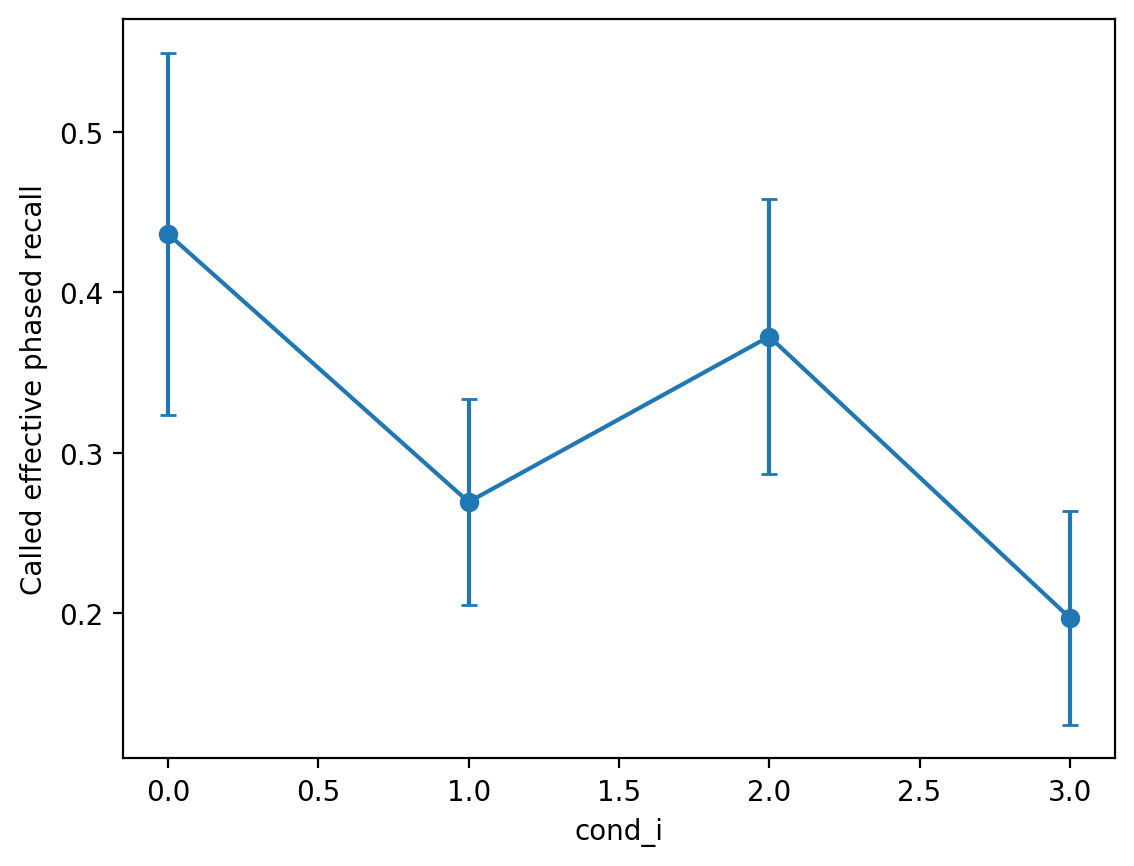
\includegraphics[width=0.82\linewidth]{figures/10_experiments/fig_10_8_2_called_effective_phased_recall.png}
\end{center}

\textbf{Figure 10.8.2 --- Called effective phased recall across
duplication × dropout conditions.} The combined duplication + dropout
condition produces the lowest end-to-end phased recall, showing that the
two stressors interact to create a substantially more difficult phasing
problem than either one alone.

\textbf{Figure 10.8.3 --- Called number of phase sets across duplication
× dropout conditions.}\\
Phase fragmentation is driven primarily by dropout, but remains high in
the combined condition. This indicates that low-coverage gaps are the
main cause of broken block continuity, while duplication compounds the
end-to-end difficulty in other ways.

\textbf{Figure 10.8.4 --- Called switch error across duplication ×
dropout conditions.}\\
Switch error should be interpreted cautiously in the interaction study.
Although duplication alone produces the highest switch error, the
combined condition is much more fragmented and leaves fewer phased
adjacencies to compare, making completeness and fragmentation metrics
more informative than switch error alone.

\subsubsection{Results summary (means over
seeds)}\label{results-summary-means-over-seeds-6}

\begin{itemize}
\tightlist
\item
  \texttt{call\_recall}:

  \begin{itemize}
  \tightlist
  \item
    \texttt{dup=0,\ dropout=0.0}: 0.663
  \item
    \texttt{dup=0,\ dropout=0.1}: 0.605
  \item
    \texttt{dup=5,\ dropout=0.0}: 0.666
  \item
    \texttt{dup=5,\ dropout=0.1}: 0.582
  \end{itemize}
\item
  \texttt{oracle\_effective\_phased\_recall}:

  \begin{itemize}
  \tightlist
  \item
    0.925 → 0.857 → 0.918 → 0.847
  \end{itemize}
\item
  \texttt{oracle\_num\_phase\_sets}:

  \begin{itemize}
  \tightlist
  \item
    1.8 → 3.2 → 1.8 → 4.0
  \end{itemize}
\item
  \texttt{called\_effective\_phased\_recall}:

  \begin{itemize}
  \tightlist
  \item
    0.436 → 0.269 → 0.373 → 0.197
  \end{itemize}
\item
  \texttt{called\_shared\_het\_recall}:

  \begin{itemize}
  \tightlist
  \item
    0.590 → 0.529 → 0.593 → 0.501
  \end{itemize}
\item
  \texttt{called\_phasing\_rate\_shared\_het}:

  \begin{itemize}
  \tightlist
  \item
    0.819 → 0.514 → 0.778 → 0.410
  \end{itemize}
\item
  \texttt{called\_phase\_accuracy}:

  \begin{itemize}
  \tightlist
  \item
    0.890 → 0.981 → 0.802 → 0.940
  \end{itemize}
\item
  \texttt{called\_switch\_error}:

  \begin{itemize}
  \tightlist
  \item
    0.122 → 0.006 → 0.207 → 0.062
  \end{itemize}
\item
  \texttt{called\_num\_phase\_sets}:

  \begin{itemize}
  \tightlist
  \item
    3.4 → 6.2 → 2.6 → 6.2
  \end{itemize}
\end{itemize}

Taken together, these results show that the combined duplication +
dropout condition is substantially worse than either single stressor
alone, and that the strongest compounded loss occurs in the called
regime rather than in the oracle regime.

\subsubsection{Key observations}\label{key-observations-6}

\begin{itemize}
\item
  O1 (The combined condition is the worst end-to-end setting): Called
  effective phased recall decreases from \texttt{0.436} in the baseline
  to \texttt{0.269} with dropout alone, \texttt{0.373} with duplication
  alone, and \texttt{0.197} when both stressors are combined. This shows
  that duplication and dropout together create a materially more
  difficult end-to-end phasing condition than either stressor in
  isolation.
\item
  O2 (Dropout remains the main driver of phasing fragmentation): In the
  oracle regime, duplication alone has little effect
  (\texttt{oracle\_num\_phase\_sets\ =\ 1.8}), whereas dropout increases
  fragmentation (\texttt{1.8\ →\ 3.2}) and the combined condition
  increases it further (\texttt{4.0}). This indicates that coverage gaps
  are the primary cause of broken phase-block connectivity.
\item
  O3 (The interaction is strongest in the called regime): Relative to
  dropout alone, the combined condition further reduces
  \texttt{call\_recall} (\texttt{0.605\ →\ 0.582}),
  \texttt{called\_shared\_het\_recall} (\texttt{0.529\ →\ 0.501}), and
  \texttt{called\_phasing\_rate\_shared\_het}
  (\texttt{0.514\ →\ 0.410}). This shows that duplication compounds
  dropout by worsening both variant recovery and phasing completeness on
  surviving shared heterozygous sites.
\item
  O4 (The compounded weakness is mixed rather than purely
  phaser-limited): Oracle effective phased recall decreases only
  modestly from \texttt{0.857} to \texttt{0.847} when duplication is
  added on top of dropout, but called effective phased recall decreases
  more substantially from \texttt{0.269} to \texttt{0.197}. Therefore,
  the main interaction effect is not purely within phasing itself; it
  arises more strongly from the end-to-end combination of reduced
  callable overlap and weaker phasing connectivity.
\item
  O5 (Switch error is not the main interaction signal): Although
  duplication alone produces the highest called switch error, the
  combined condition does not. This should not be interpreted as an
  improvement, because the combined condition is much more fragmented
  and leaves fewer adjacent phased heterozygous pairs to compare. In
  this interaction study, completeness and fragmentation metrics are
  more informative than switch error alone.
\end{itemize}

\subsubsection{Optimization implication}\label{optimization-implication}

The duplication × dropout interaction suggests that the most important
optimization opportunities under compounded stress are not limited to
WhatsHap read selection. Preserving phasing evidence remains important
(e.g., avoiding overly strict \texttt{min\_baseq} filtering), but the
interaction also indicates that upstream variant recovery in ambiguous
and low-coverage regions is a major limiting factor. This motivates
future tuning of calling-side thresholds and, potentially, more
region-aware handling of ambiguous reads near coverage gaps.

\subsubsection{Takeaway}\label{takeaway-6}

Duplicated regions and coverage dropout interact to produce a more
severe end-to-end phasing weakness than either stressor alone. Dropout
drives fragmentation, while duplication further reduces callable overlap
and phasing completeness in the called regime. This makes the
interaction a useful diagnostic for optimization: it shows that
practical improvements will likely require both careful preservation of
phasing evidence and better upstream handling of difficult regions,
rather than relying on a single WhatsHap parameter alone.

\begin{center}\rule{0.5\linewidth}{0.5pt}\end{center}

\subsection{10.9 Optimization sweeps (WhatsHap / pipeline
parameters)}\label{optimization-sweeps-whatshap-pipeline-parameters}

\subsubsection{Aim}\label{aim-7}

Identify parameter settings that improve phasing performance under a
composite hard scenario, and quantify trade-offs between phased recall,
switch error, fragmentation, and robustness.

\subsubsection{Hard scenario}\label{hard-scenario}

Optimization sweeps were conducted on a fixed composite stress condition
designed to combine several realism knobs: - duplicated regions
(\texttt{dup\_segments\ =\ 5}) - coverage dropout
(\texttt{dropout\_fraction\ =\ 0.1},
\texttt{dropout\_block\_len\ =\ 1000}) - correlated error bursts
(\texttt{burst\_prob\ =\ 0.6}, \texttt{burst\_count\ =\ 2},
\texttt{burst\_len\ =\ 300}, \texttt{burst\_mult\ =\ 8.0}) - truth
indels (\texttt{num\_indels\ =\ 120}, SNP-only phasing/evaluation
enabled) - \texttt{ref\_length\ =\ 120\ kb} -
\texttt{num\_snps\ =\ 1200} - \texttt{num\_reads\ =\ 300}

This hard scenario was chosen to test whether WhatsHap-side tuning can
recover performance under combined realistic stresses rather than under
isolated perturbations.

\subsubsection{\texorpdfstring{10.9.1 Sweep A:
\texttt{max\_coverage}}{10.9.1 Sweep A: max\_coverage}}\label{sweep-a-max_coverage}

\paragraph{Setup}\label{setup-7}

\begin{itemize}
\tightlist
\item
  Varied: \texttt{max\_coverage\ ∈\ \{10,\ 15,\ 25,\ 40\}}
\item
  Fixed: all other hard-scenario parameters
\end{itemize}

\paragraph{Figures to include}\label{figures-to-include-7}

\begin{itemize}
\tightlist
\item
  \textbf{Figure 10.9.1.1 --- Called effective phased recall vs
  \texttt{max\_coverage}.}
\item
  \textbf{Figure 10.9.1.2 --- Called switch error vs
  \texttt{max\_coverage}.}
\item
  \textbf{Figure 10.9.1.3 --- Called number of phase sets vs
  \texttt{max\_coverage}.}
\item
  \textbf{Figure 10.9.1.4 --- Total pipeline runtime vs
  \texttt{max\_coverage}.}
\end{itemize}

\textbf{Figure 10.9.1.1 --- Called effective phased recall vs
\texttt{max\_coverage}.}\\
Called effective phased recall remains essentially flat across the
\texttt{max\_coverage} sweep, indicating that increasing the WhatsHap
read-selection cap does not provide a meaningful gain under the current
hard scenario.

\textbf{Figure 10.9.1.2 --- Called switch error vs
\texttt{max\_coverage}.}\\
Called switch error shows no meaningful dependence on
\texttt{max\_coverage}, further indicating that read-selection depth is
not the limiting factor for phasing correctness in the current hard
scenario.

\textbf{Figure 10.9.1.3 --- Called number of phase sets vs
\texttt{max\_coverage}.}\\
Phase-set fragmentation remains unchanged across the
\texttt{max\_coverage} sweep, showing that retaining more reads does not
improve haplotype continuity in this stress condition.

\textbf{Figure 10.9.1.4 --- Total pipeline runtime vs
\texttt{max\_coverage}.}\\
Runtime increases substantially as \texttt{max\_coverage} increases, but
phasing performance remains nearly unchanged. This indicates that higher
\texttt{max\_coverage} mainly adds compute cost rather than practical
benefit.

\paragraph{Results summary}\label{results-summary}

\begin{itemize}
\tightlist
\item
  \texttt{call\_recall}: 0.5895 at all \texttt{max\_coverage} settings
\item
  \texttt{called\_effective\_phased\_recall}: 0.2917 → 0.2919 → 0.2919 →
  0.2919
\item
  \texttt{called\_switch\_error}: 0.0056 at all \texttt{max\_coverage}
  settings
\item
  \texttt{called\_num\_phase\_sets}: 9.6 at all \texttt{max\_coverage}
  settings
\item
  \texttt{called\_shared\_het\_recall}: 0.5098 at all
  \texttt{max\_coverage} settings
\item
  \texttt{called\_phasing\_rate\_shared\_het}: 0.5860 → 0.5864 → 0.5864
  → 0.5864
\item
  \texttt{called\_phase\_accuracy}: 0.9748 at all \texttt{max\_coverage}
  settings
\item
  \texttt{oracle\_effective\_phased\_recall}: 0.8256 → 0.8298 → 0.8300 →
  0.8300
\item
  \texttt{oracle\_num\_phase\_sets}: 6.4 → 6.2 → 6.2 → 6.2
\item
  \texttt{time\_total\_sec}: 3.76 → 4.37 → 6.30 → 6.39
\end{itemize}

\paragraph{Key observations}\label{key-observations-7}

\begin{itemize}
\item
  O1 (Changing \texttt{max\_coverage} has almost no effect on phasing
  performance): Called effective phased recall, switch error, phase-set
  count, and phasing-rate-on-shared-hets remain essentially unchanged
  across the full \texttt{max\_coverage} sweep.
\item
  O2 (Runtime increases without measurable accuracy gain): Total runtime
  increases substantially as \texttt{max\_coverage} increases, but this
  additional compute does not translate into improved end-to-end phasing
  metrics.
\item
  O3 (The read-selection cap is not the active bottleneck in this hard
  scenario): Although higher \texttt{max\_coverage} retains more reads
  internally, the resulting phasing output is almost identical. This
  indicates that the limiting factor is not insufficient retained read
  coverage at the phasing stage.
\item
  O4 (Optimization headroom from \texttt{max\_coverage} is negligible):
  Under the current hard scenario, increasing the WhatsHap
  read-selection cap does not provide a practically useful optimization
  lever.
\end{itemize}

\paragraph{Takeaway}\label{takeaway-7}

Adjusting \texttt{max\_coverage} does not provide a meaningful
optimization benefit under the composite hard scenario. Since phasing
metrics remain flat while runtime increases, the default or lower
\texttt{max\_coverage} setting is preferable on efficiency grounds.

\subsubsection{\texorpdfstring{10.9.2 Sweep B: phasing quality
thresholds
(\texttt{min\_mapq\ ×\ min\_baseq})}{10.9.2 Sweep B: phasing quality thresholds (min\_mapq × min\_baseq)}}\label{sweep-b-phasing-quality-thresholds-min_mapq-min_baseq}

\paragraph{Setup}\label{setup-8}

\begin{itemize}
\tightlist
\item
  Varied:

  \begin{itemize}
  \tightlist
  \item
    \texttt{min\_mapq\ ∈\ \{0,\ 10,\ 20\}}
  \item
    \texttt{min\_baseq\ ∈\ \{0,\ 10,\ 20\}}
  \end{itemize}
\item
  Fixed: all other hard-scenario parameters
\end{itemize}

\paragraph{Figures to include}\label{figures-to-include-8}

\begin{itemize}
\tightlist
\item
  \textbf{Figure 10.9.2.1 --- Called effective phased recall across the
  \texttt{min\_mapq\ ×\ min\_baseq} grid.}
\item
  \textbf{Figure 10.9.2.2 --- Called switch error across the
  \texttt{min\_mapq\ ×\ min\_baseq} grid.}
\item
  \textbf{Figure 10.9.2.3 --- Called number of phase sets across the
  phasing quality-threshold grid (heatmap).}
\item
  \textbf{Figure 10.9.2.4 --- Oracle effective phased recall across the
  phasing quality-threshold grid (heatmap).}
\end{itemize}

\textbf{Figure 10.9.2.1 --- Called effective phased recall across the
\texttt{min\_mapq\ ×\ min\_baseq} grid.}\\
Called effective phased recall is consistently higher when
\texttt{min\_baseq\ =\ 0} or \texttt{10} than when
\texttt{min\_baseq\ =\ 20}, while \texttt{min\_mapq} has little visible
effect. This shows that overly strict base-quality filtering reduces
usable phasing evidence.

\textbf{Figure 10.9.2.2 --- Called switch error across the
\texttt{min\_mapq\ ×\ min\_baseq} grid.}\\
Called switch error is lowest when \texttt{min\_baseq\ =\ 0} or
\texttt{10} and higher when \texttt{min\_baseq\ =\ 20}, indicating that
stricter base-quality filtering does not improve phasing correctness in
this hard scenario and instead weakens phasing evidence.

\textbf{Figure 10.9.2.3 --- Called number of phase sets across the
\texttt{min\_mapq\ ×\ min\_baseq} grid.}\\
Phase fragmentation is substantially lower when
\texttt{min\_baseq\ =\ 0} or \texttt{10} than when
\texttt{min\_baseq\ =\ 20}, showing that strict base-quality filtering
breaks block continuity by removing informative allele observations.

\textbf{Figure 10.9.2.4 --- Oracle effective phased recall across the
\texttt{min\_mapq\ ×\ min\_baseq} grid.}\\
Oracle phasing performance is markedly worse when
\texttt{min\_baseq\ =\ 20}, confirming that the main threshold effect
arises within the phasing stage itself rather than through changes in
the upstream callset.

\paragraph{Results summary}\label{results-summary-1}

\begin{itemize}
\tightlist
\item
  For \texttt{min\_baseq\ =\ 0\ or\ 10}:

  \begin{itemize}
  \tightlist
  \item
    \texttt{called\_effective\_phased\_recall}: 0.2964
  \item
    \texttt{called\_switch\_error}: 0.0007
  \item
    \texttt{called\_num\_phase\_sets}: 6.6
  \item
    \texttt{called\_phasing\_rate\_shared\_het}: 0.6027
  \item
    \texttt{oracle\_effective\_phased\_recall}: 0.9402--0.9415
  \item
    \texttt{oracle\_num\_phase\_sets}: 3.8
  \end{itemize}
\item
  For \texttt{min\_baseq\ =\ 20}:

  \begin{itemize}
  \tightlist
  \item
    \texttt{called\_effective\_phased\_recall}: 0.2919--0.2923
  \item
    \texttt{called\_switch\_error}: 0.0056
  \item
    \texttt{called\_num\_phase\_sets}: 9.6
  \item
    \texttt{called\_phasing\_rate\_shared\_het}: 0.5864--0.5872
  \item
    \texttt{oracle\_effective\_phased\_recall}: 0.8298--0.8319
  \item
    \texttt{oracle\_num\_phase\_sets}: 6.2--6.4
  \end{itemize}
\item
  \texttt{min\_mapq} has negligible effect across the grid.
\item
  \texttt{call\_recall} remains constant at 0.5895 because
  variant-calling thresholds are fixed and only phasing-side filters are
  varied here.
\end{itemize}

\paragraph{Key observations}\label{key-observations-8}

\begin{itemize}
\item
  O1 (Base-quality filtering is the main useful phasing-side knob): The
  grid separates into two clear regimes. Using
  \texttt{min\_baseq\ =\ 0\ or\ 10} improves called effective phased
  recall, lowers switch error, and reduces phase fragmentation relative
  to \texttt{min\_baseq\ =\ 20}.
\item
  O2 (Overly strict \texttt{min\_baseq} harms both oracle and called
  phasing): Raising \texttt{min\_baseq} to 20 reduces oracle effective
  phased recall from about \texttt{0.94} to about \texttt{0.83}, and
  increases oracle phase-set count from \texttt{3.8} to
  \texttt{6.2–6.4}. This shows that strict base-quality filtering
  discards too much informative phasing evidence.
\item
  O3 (\texttt{min\_mapq} contributes little under the current hard
  scenario): Changing \texttt{min\_mapq} from 0 to 20 produces almost no
  measurable difference in called or oracle metrics, indicating that
  mapping-quality filtering is not a strong optimization lever here.
\item
  O4 (The gain from threshold tuning is modest but real): Lowering
  \texttt{min\_baseq} improves phasing completeness and continuity, but
  the absolute gain in called effective phased recall is still small
  because the dominant loss term remains missing shared heterozygous
  sites.
\end{itemize}

\paragraph{Takeaway}\label{takeaway-8}

Phasing quality thresholds provide a limited but real optimization lever
under the composite hard scenario. The most useful change is to avoid
overly strict base-quality filtering: \texttt{min\_baseq\ =\ 10} (or 0)
clearly outperforms \texttt{min\_baseq\ =\ 20}, while \texttt{min\_mapq}
has little practical impact.

\subsubsection{\texorpdfstring{10.9.3 Sweep C: calling thresholds
(\texttt{call\_min\_mapq\ ×\ call\_min\_baseq})}{10.9.3 Sweep C: calling thresholds (call\_min\_mapq × call\_min\_baseq)}}\label{sweep-c-calling-thresholds-call_min_mapq-call_min_baseq}

\paragraph{Setup}\label{setup-9}

\begin{itemize}
\tightlist
\item
  Varied:

  \begin{itemize}
  \tightlist
  \item
    \texttt{call\_min\_mapq\ ∈\ \{0,\ 10,\ 20\}}
  \item
    \texttt{call\_min\_baseq\ ∈\ \{5,\ 10,\ 15,\ 20\}}
  \end{itemize}
\item
  Fixed:

  \begin{itemize}
  \tightlist
  \item
    hard-scenario stressors unchanged
  \item
    phasing parameters fixed to the best practical settings identified
    earlier:

    \begin{itemize}
    \tightlist
    \item
      \texttt{max\_coverage\ =\ 10}
    \item
      \texttt{min\_mapq\ =\ 20}
    \item
      \texttt{min\_baseq\ =\ 10}
    \end{itemize}
  \end{itemize}
\end{itemize}

\paragraph{Figures to include}\label{figures-to-include-9}

\begin{itemize}
\tightlist
\item
  \textbf{Figure 10.9.3.1 --- Variant calling recall across the
  caller-threshold grid (heatmap).}
\item
  \textbf{Figure 10.9.3.2 --- Called effective phased recall across the
  \texttt{call\_min\_mapq\ ×\ call\_min\_baseq} grid.}
\item
  \textbf{Figure 10.9.3.3 --- Called shared heterozygous recall across
  the \texttt{call\_min\_mapq\ ×\ call\_min\_baseq} grid.}
\item
  \textbf{Figure 10.9.3.4 --- Call precision across the
  \texttt{call\_min\_mapq\ ×\ call\_min\_baseq} grid.}
\end{itemize}

\textbf{Figure 10.9.3.1 --- Calling recall across the
\texttt{call\_min\_mapq\ ×\ call\_min\_baseq} grid.}\\
Calling recall depends strongly on \texttt{call\_min\_baseq} but only
weakly on \texttt{call\_min\_mapq}. Moderate base-quality thresholds
retain more true SNP evidence, whereas \texttt{call\_min\_baseq\ =\ 20}
is overly strict and sharply reduces variant recovery.

\textbf{Figure 10.9.3.2 --- Called effective phased recall across the
\texttt{call\_min\_mapq\ ×\ call\_min\_baseq} grid.}\\
End-to-end phased recall is highest when \texttt{call\_min\_baseq\ =\ 5}
or \texttt{10}, showing that caller-side base-quality filtering has a
direct downstream impact on usable phasing performance.

\textbf{Figure 10.9.3.3 --- Called shared heterozygous recall across the
\texttt{call\_min\_mapq\ ×\ call\_min\_baseq} grid.}\\
Called shared heterozygous recall follows the same pattern as calling
recall, indicating that the main benefit of moderate caller thresholds
is better recovery of true heterozygous SNPs that can subsequently be
phased.

\textbf{Figure 10.9.3.4 --- Call precision across the
\texttt{call\_min\_mapq\ ×\ call\_min\_baseq} grid.}\\
Call precision remains very high across the full threshold grid, showing
that the gains from moderate caller base-quality thresholds are achieved
without a substantial precision penalty.

\paragraph{Results summary}\label{results-summary-2}

\begin{itemize}
\tightlist
\item
  For \texttt{call\_min\_baseq\ =\ 5\ or\ 10}:

  \begin{itemize}
  \tightlist
  \item
    \texttt{call\_precision}: \textasciitilde0.9995
  \item
    \texttt{call\_recall}: \textasciitilde0.596--0.597
  \item
    \texttt{called\_shared\_het\_recall}: \textasciitilde0.517--0.518
  \item
    \texttt{called\_effective\_phased\_recall}:
    \textasciitilde0.3155--0.3157
  \item
    \texttt{called\_phasing\_rate\_shared\_het}:
    \textasciitilde0.609--0.610
  \item
    \texttt{called\_switch\_error}: 0.0000
  \item
    \texttt{called\_num\_phase\_sets}: 6.6
  \end{itemize}
\item
  For \texttt{call\_min\_baseq\ =\ 15}:

  \begin{itemize}
  \tightlist
  \item
    \texttt{call\_recall}: \textasciitilde0.589--0.590
  \item
    \texttt{called\_shared\_het\_recall}: \textasciitilde0.509--0.510
  \item
    \texttt{called\_effective\_phased\_recall}:
    \textasciitilde0.307--0.3074
  \end{itemize}
\item
  For \texttt{call\_min\_baseq\ =\ 20}:

  \begin{itemize}
  \tightlist
  \item
    \texttt{call\_precision}: \textasciitilde0.9991
  \item
    \texttt{call\_recall}: \textasciitilde0.3645--0.3647
  \item
    \texttt{called\_shared\_het\_recall}: \textasciitilde0.287
  \item
    \texttt{called\_effective\_phased\_recall}:
    \textasciitilde0.1144--0.1146
  \item
    \texttt{called\_phasing\_rate\_shared\_het}: \textasciitilde0.399
  \item
    \texttt{called\_num\_phase\_sets}: 7.0
  \end{itemize}
\item
  \texttt{call\_min\_mapq} has negligible effect across the grid.
\end{itemize}

\paragraph{Key observations}\label{key-observations-9}

\begin{itemize}
\item
  O1 (Caller base-quality filtering is a strong optimization lever):
  Lowering \texttt{call\_min\_baseq} from 20 to 10 or 5 substantially
  improves call recall, called shared-heterozygous recall, and called
  effective phased recall. This shows that overly strict caller
  base-quality filtering removes too much useful variant evidence under
  the composite hard scenario.
\item
  O2 (Caller mapping-quality filtering has little practical effect):
  Changing \texttt{call\_min\_mapq} from 0 to 20 produces almost no
  measurable difference in calling or phasing metrics. Under the current
  hard scenario, base-quality filtering is therefore the dominant
  caller-side threshold knob.
\item
  O3 (The gain arises through overlap recovery rather than phasing
  correctness): Oracle effective phased recall remains fixed
  (\textasciitilde0.9402), while called phase accuracy and switch error
  remain near-perfect in the best settings. This indicates that the
  improvement comes mainly from recovering more true shared heterozygous
  sites rather than from changing phasing correctness itself.
\item
  O4 (Moderate caller thresholds outperform strict thresholds without
  sacrificing precision): The best-performing settings
  (\texttt{call\_min\_baseq\ =\ 5\ or\ 10}) retain very high call
  precision (\textasciitilde0.9995) while increasing end-to-end phased
  recall. This makes moderate caller base-quality thresholds a practical
  optimization opportunity in this pipeline.
\end{itemize}

\paragraph{Takeaway}\label{takeaway-9}

Calling thresholds provide a more effective optimization lever than the
WhatsHap-only sweeps tested earlier. In particular, a moderate caller
base-quality threshold (\texttt{call\_min\_baseq\ =\ 10}, or 5) improves
variant recovery and end-to-end phased recall without materially harming
precision, while \texttt{call\_min\_baseq\ =\ 20} is clearly too strict
under the current hard scenario.

\subsubsection{\texorpdfstring{10.9.4 Sweep D: runtime-focused lower
\texttt{max\_coverage}}{10.9.4 Sweep D: runtime-focused lower max\_coverage}}\label{sweep-d-runtime-focused-lower-max_coverage}

\paragraph{Setup}\label{setup-10}

\begin{itemize}
\tightlist
\item
  Varied: \texttt{max\_coverage\ ∈\ \{4,\ 6,\ 8,\ 10,\ 15\}}
\item
  Fixed:

  \begin{itemize}
  \tightlist
  \item
    hard-scenario stressors unchanged
  \item
    caller thresholds fixed to a strong practical setting:

    \begin{itemize}
    \tightlist
    \item
      \texttt{call\_min\_mapq\ =\ 20}
    \item
      \texttt{call\_min\_baseq\ =\ 15}
    \end{itemize}
  \item
    phasing thresholds fixed to the best practical settings identified
    earlier:

    \begin{itemize}
    \tightlist
    \item
      \texttt{min\_mapq\ =\ 20}
    \item
      \texttt{min\_baseq\ =\ 10}
    \end{itemize}
  \end{itemize}
\end{itemize}

\paragraph{Figures to include}\label{figures-to-include-10}

\begin{itemize}
\tightlist
\item
  \textbf{Figure 10.9.4.1 --- Called effective phased recall vs lower
  \texttt{max\_coverage}.}
\item
  \textbf{Figure 10.9.4.2 --- Called number of phase sets vs lower
  \texttt{max\_coverage}.}
\item
  \textbf{Figure 10.9.4.3 --- Oracle effective phased recall vs lower
  \texttt{max\_coverage}.}
\item
  \textbf{Figure 10.9.4.4 --- Total pipeline runtime vs lower
  \texttt{max\_coverage}.}
\end{itemize}

\textbf{Figure 10.9.4.1 --- Called effective phased recall vs lower
\texttt{max\_coverage}.}\\
Called effective phased recall is essentially unchanged for
\texttt{max\_coverage\ =\ 8,\ 10,\ 15}, indicating that retained phasing
coverage above 8 provides no practical benefit in the current hard
scenario.

\textbf{Figure 10.9.4.2 --- Called number of phase sets vs lower
\texttt{max\_coverage}.}\\
Phase fragmentation is stable from \texttt{max\_coverage\ =\ 6} upward,
but becomes slightly worse at \texttt{max\_coverage\ =\ 4}, suggesting
that very aggressive down-selection can begin to remove useful
connectivity.

\textbf{Figure 10.9.4.3 --- Oracle effective phased recall vs lower
\texttt{max\_coverage}.}\\
Oracle phasing performance improves slightly from
\texttt{max\_coverage\ =\ 4} to \texttt{8}, then plateaus. This
indicates that a small amount of retained coverage is necessary for full
phasing continuity, but higher retained coverage beyond 8 is
unnecessary.

\textbf{Figure 10.9.4.4 --- Total pipeline runtime vs lower
\texttt{max\_coverage}.}\\
Runtime is similar for \texttt{max\_coverage\ =\ 6–10} but increases
noticeably at \texttt{15}, showing that a lower retained-coverage cap
can reduce compute cost without sacrificing phasing performance.

\paragraph{Results summary}\label{results-summary-3}

\begin{itemize}
\tightlist
\item
  \texttt{call\_recall}: 0.5895 at all \texttt{max\_coverage} settings
\item
  \texttt{call\_precision}: 0.9994 at all \texttt{max\_coverage}
  settings
\item
  \texttt{called\_effective\_phased\_recall}:

  \begin{itemize}
  \tightlist
  \item
    0.2958 (\texttt{max\_coverage\ =\ 4})
  \item
    0.2960 (\texttt{6})
  \item
    0.2964 (\texttt{8})
  \item
    0.2964 (\texttt{10})
  \item
    0.2964 (\texttt{15})
  \end{itemize}
\item
  \texttt{called\_switch\_error}:

  \begin{itemize}
  \tightlist
  \item
    0.0051 → 0.0038 → 0.0007 → 0.0007 → 0.0007
  \end{itemize}
\item
  \texttt{called\_num\_phase\_sets}:

  \begin{itemize}
  \tightlist
  \item
    6.8 → 6.6 → 6.6 → 6.6 → 6.6
  \end{itemize}
\item
  \texttt{called\_phase\_accuracy}:

  \begin{itemize}
  \tightlist
  \item
    0.9604 → 0.9610 → 0.9625 → 0.9625 → 0.9625
  \end{itemize}
\item
  \texttt{oracle\_effective\_phased\_recall}:

  \begin{itemize}
  \tightlist
  \item
    0.9228 → 0.9348 → 0.9402 → 0.9402 → 0.9402
  \end{itemize}
\item
  \texttt{oracle\_num\_phase\_sets}:

  \begin{itemize}
  \tightlist
  \item
    5.0 → 3.8 → 3.8 → 3.8 → 3.8
  \end{itemize}
\item
  \texttt{time\_total\_sec}:

  \begin{itemize}
  \tightlist
  \item
    3.6877 → 3.6720 → 3.6769 → 3.6774 → 4.2029
  \end{itemize}
\end{itemize}

\paragraph{Key observations}\label{key-observations-10}

\begin{itemize}
\item
  O1 (Performance plateaus by \texttt{max\_coverage\ =\ 8}): Called
  effective phased recall, switch error, phase-set count, and phase
  accuracy are essentially identical for
  \texttt{max\_coverage\ =\ 8,\ 10,\ 15}. This shows that retained
  phasing coverage above 8 does not provide additional practical benefit
  under the current hard scenario.
\item
  O2 (Very low \texttt{max\_coverage} begins to hurt modestly): At
  \texttt{max\_coverage\ =\ 4}, oracle effective phased recall and
  oracle continuity are slightly worse, and called metrics are also
  marginally lower. This suggests that reducing retained coverage too
  aggressively can begin to remove useful bridging evidence.
\item
  O3 (The best efficiency region is around
  \texttt{max\_coverage\ =\ 8–10}): Runtime remains around 3.67 seconds
  for \texttt{max\_coverage\ =\ 6–10}, but increases to about 4.20
  seconds at \texttt{15} without any measurable gain in phasing
  performance.
\item
  O4 (\texttt{max\_coverage\ =\ 15} is unnecessarily expensive):
  Compared with \texttt{max\_coverage\ =\ 8–10}, the setting \texttt{15}
  increases runtime by roughly 14\% while leaving the main phasing
  metrics unchanged. This makes higher retained coverage unattractive on
  efficiency grounds.
\end{itemize}

\paragraph{Takeaway}\label{takeaway-10}

A lower \texttt{max\_coverage} setting provides a practical runtime
optimization under the composite hard scenario. The best trade-off is
around \texttt{max\_coverage\ =\ 8} or \texttt{10}, where performance is
indistinguishable from \texttt{15} but runtime is lower. In contrast,
\texttt{max\_coverage\ =\ 4} is slightly too aggressive and begins to
degrade continuity-related metrics.

\subsubsection{\texorpdfstring{10.9.5 Sweep E: fine phasing
\texttt{min\_baseq}}{10.9.5 Sweep E: fine phasing min\_baseq}}\label{sweep-e-fine-phasing-min_baseq}

\paragraph{Setup}\label{setup-11}

\begin{itemize}
\tightlist
\item
  Varied: \texttt{min\_baseq\ ∈\ \{0,\ 5,\ 10,\ 15,\ 20\}}
\item
  Fixed:

  \begin{itemize}
  \tightlist
  \item
    hard-scenario stressors unchanged
  \item
    caller thresholds fixed to a strong practical setting:

    \begin{itemize}
    \tightlist
    \item
      \texttt{call\_min\_mapq\ =\ 20}
    \item
      \texttt{call\_min\_baseq\ =\ 15}
    \end{itemize}
  \item
    phasing parameters otherwise fixed:

    \begin{itemize}
    \tightlist
    \item
      \texttt{max\_coverage\ =\ 10}
    \item
      \texttt{min\_mapq\ =\ 20}
    \end{itemize}
  \end{itemize}
\end{itemize}

\paragraph{Figures to include}\label{figures-to-include-11}

\begin{itemize}
\tightlist
\item
  \textbf{Figure 10.9.5.1 --- Called effective phased recall vs fine
  phasing \texttt{min\_baseq}.}
\item
  \textbf{Figure 10.9.5.2 --- Called number of phase sets vs fine
  phasing \texttt{min\_baseq}.}
\item
  \textbf{Figure 10.9.5.3 --- Oracle effective phased recall vs fine
  phasing \texttt{min\_baseq}.}
\item
  \textbf{Figure 10.9.5.4 --- Called switch error vs fine phasing
  \texttt{min\_baseq}.}
\end{itemize}

\textbf{Figure 10.9.5.1 --- Called effective phased recall vs fine
phasing \texttt{min\_baseq}.}\\
Called effective phased recall remains flat from
\texttt{min\_baseq\ =\ 0} to \texttt{15}, then decreases at \texttt{20},
indicating that only overly strict phasing base-quality filtering harms
usable end-to-end phasing output.

\textbf{Figure 10.9.5.2 --- Called number of phase sets vs fine phasing
\texttt{min\_baseq}.}\\
Phase fragmentation is unchanged across \texttt{min\_baseq\ =\ 0–15} but
increases substantially at \texttt{20}, showing that strict phasing
base-quality filtering breaks block continuity by discarding informative
allele observations.

\textbf{Figure 10.9.5.3 --- Oracle effective phased recall vs fine
phasing \texttt{min\_baseq}.}\\
Oracle phasing performance is stable up to \texttt{min\_baseq\ =\ 15}
and then drops sharply at \texttt{20}, confirming that the harmful
threshold effect arises within the phasing stage itself rather than
through upstream callset changes.

\textbf{Figure 10.9.5.4 --- Called switch error vs fine phasing
\texttt{min\_baseq}.}\\
Called switch error remains very low and stable from
\texttt{min\_baseq\ =\ 0} to \texttt{15}, but increases at \texttt{20},
indicating that overly strict phasing base-quality filtering weakens the
consistency of retained phasing evidence.

\paragraph{Results summary}\label{results-summary-4}

\begin{itemize}
\tightlist
\item
  \texttt{call\_recall}: 0.5895 at all \texttt{min\_baseq} settings
\item
  \texttt{call\_precision}: 0.9994 at all \texttt{min\_baseq} settings
\item
  \texttt{called\_effective\_phased\_recall}:

  \begin{itemize}
  \tightlist
  \item
    0.2964 (\texttt{min\_baseq\ =\ 0})
  \item
    0.2964 (\texttt{5})
  \item
    0.2964 (\texttt{10})
  \item
    0.2964 (\texttt{15})
  \item
    0.2917 (\texttt{20})
  \end{itemize}
\item
  \texttt{called\_switch\_error}:

  \begin{itemize}
  \tightlist
  \item
    0.0007 → 0.0007 → 0.0007 → 0.0007 → 0.0056
  \end{itemize}
\item
  \texttt{called\_num\_phase\_sets}:

  \begin{itemize}
  \tightlist
  \item
    6.6 → 6.6 → 6.6 → 6.6 → 9.6
  \end{itemize}
\item
  \texttt{called\_phase\_accuracy}:

  \begin{itemize}
  \tightlist
  \item
    0.9625 → 0.9625 → 0.9625 → 0.9625 → 0.9748
  \end{itemize}
\item
  \texttt{oracle\_effective\_phased\_recall}:

  \begin{itemize}
  \tightlist
  \item
    0.9402 → 0.9402 → 0.9402 → 0.9375 → 0.8256
  \end{itemize}
\item
  \texttt{oracle\_num\_phase\_sets}:

  \begin{itemize}
  \tightlist
  \item
    3.8 → 3.8 → 3.8 → 3.8 → 6.4
  \end{itemize}
\item
  \texttt{time\_total\_sec}:

  \begin{itemize}
  \tightlist
  \item
    3.6758 → 3.6505 → 3.6501 → 3.6172 → 3.6158
  \end{itemize}
\end{itemize}

\paragraph{Key observations}\label{key-observations-11}

\begin{itemize}
\item
  O1 (Phasing performance is flat from \texttt{min\_baseq\ =\ 0} to
  \texttt{15}): Called effective phased recall, switch error, phase-set
  count, and phase accuracy are effectively identical across
  \texttt{min\_baseq\ ∈\ \{0,\ 5,\ 10,\ 15\}}. This indicates that
  moderate variation in phasing base-quality filtering has no measurable
  effect within this range.
\item
  O2 (The harmful threshold is \texttt{min\_baseq\ =\ 20}): Raising
  \texttt{min\_baseq} to 20 reduces called effective phased recall,
  increases switch error, and increases phase fragmentation. Oracle
  effective phased recall also drops sharply
  (\texttt{0.9402\ →\ 0.8256}), confirming that the loss is caused
  within the phasing stage itself.
\item
  O3 (There is no practical benefit to using values below 10): Since
  \texttt{0}, \texttt{5}, and \texttt{10} perform identically, more
  permissive phasing base-quality thresholds do not yield additional
  measurable gains under the current hard scenario.
\item
  O4 (\texttt{min\_baseq\ =\ 10} is the best practical recommendation):
  Because \texttt{10} lies on the same performance plateau as
  \texttt{0}, \texttt{5}, and \texttt{15}, but is easier to justify as a
  moderate threshold, it provides the cleanest practical phasing setting
  for the remainder of the study.
\end{itemize}

\paragraph{Takeaway}\label{takeaway-11}

The fine phasing \texttt{min\_baseq} sweep confirms that performance is
stable across \texttt{min\_baseq\ =\ 0–15} and degrades only when the
threshold becomes too strict (\texttt{20}). A moderate phasing
base-quality threshold such as \texttt{min\_baseq\ =\ 10} is therefore
the most practical recommendation: it retains full performance while
avoiding unnecessary permissiveness and clearly outperforming the overly
strict setting.

\subsubsection{10.9.6 Default vs optimized
comparison}\label{default-vs-optimized-comparison}

\paragraph{Setup}\label{setup-12}

A final confirmation run compared the default hard-scenario
configuration against the best practical tuned configuration identified
from the preceding optimization sweeps.

\begin{itemize}
\tightlist
\item
  \textbf{Default configuration}

  \begin{itemize}
  \tightlist
  \item
    \texttt{call\_min\_mapq\ =\ 20}
  \item
    \texttt{call\_min\_baseq\ =\ 15}
  \item
    \texttt{max\_coverage\ =\ 15}
  \item
    \texttt{min\_mapq\ =\ 20}
  \item
    \texttt{min\_baseq\ =\ 20}
  \end{itemize}
\item
  \textbf{Optimized configuration}

  \begin{itemize}
  \tightlist
  \item
    \texttt{call\_min\_mapq\ =\ 20}
  \item
    \texttt{call\_min\_baseq\ =\ 10}
  \item
    \texttt{max\_coverage\ =\ 8}
  \item
    \texttt{min\_mapq\ =\ 20}
  \item
    \texttt{min\_baseq\ =\ 10}
  \end{itemize}
\end{itemize}

All other hard-scenario stressors were kept fixed.

\paragraph{Figures to include}\label{figures-to-include-12}

\begin{itemize}
\tightlist
\item
  \textbf{Figure 10.9.6.1 --- Called effective phased recall: default vs
  optimized.}
\item
  \textbf{Figure 10.9.6.2 --- Called shared heterozygous recall: default
  vs optimized.}
\item
  \textbf{Figure 10.9.6.3 --- Called number of phase sets: default vs
  optimized.}
\item
  \textbf{Figure 10.9.6.4 --- Total pipeline runtime: default vs
  optimized.}
\end{itemize}

\textbf{Figure 10.9.6.1 --- Called effective phased recall: default vs
optimized.}\\
The optimized configuration achieves higher end-to-end phased recall
than the default hard-scenario setting, confirming that coordinated
parameter tuning yields a measurable improvement under compounded
realistic stress.

\textbf{Figure 10.9.6.2 --- Called shared heterozygous recall: default
vs optimized.}\\
The optimized configuration increases called shared heterozygous recall,
indicating that part of the improvement comes from recovering more true
heterozygous sites that can subsequently be phased.

\textbf{Figure 10.9.6.3 --- Called number of phase sets: default vs
optimized.}\\
The optimized configuration substantially reduces the number of phase
sets, showing that it preserves stronger phase-block continuity than the
default setting under the hard scenario.

\textbf{Figure 10.9.6.4 --- Total pipeline runtime: default vs
optimized.}\\
The optimized configuration is slightly faster than the default while
also improving phasing performance, showing that the observed gains are
not achieved at the cost of higher compute.

\paragraph{Results summary}\label{results-summary-5}

Means over 5 seeds:

\begin{itemize}
\tightlist
\item
  \texttt{time\_total\_sec}: 4.0614 → 3.9783
\item
  \texttt{call\_precision}: 0.9994 → 0.9995
\item
  \texttt{call\_recall}: 0.5895 → 0.5970
\item
  \texttt{oracle\_effective\_phased\_recall}: 0.8298 → 0.9402
\item
  \texttt{oracle\_switch\_error}: 0.0083 → 0.0031
\item
  \texttt{oracle\_num\_phase\_sets}: 6.2 → 3.8
\item
  \texttt{called\_effective\_phased\_recall}: 0.2919 → 0.3041
\item
  \texttt{called\_shared\_het\_recall}: 0.5098 → 0.5181
\item
  \texttt{called\_phasing\_rate\_shared\_het}: 0.5864 → 0.6090
\item
  \texttt{called\_phase\_accuracy}: 0.9748 → 0.9622
\item
  \texttt{called\_switch\_error}: 0.0056 → 0.0007
\item
  \texttt{called\_num\_phase\_sets}: 9.6 → 6.6
\end{itemize}

\paragraph{Key observations}\label{key-observations-12}

\begin{itemize}
\item
  O1 (The optimized configuration improves end-to-end phased recall):
  Called effective phased recall increases from \texttt{0.2919} to
  \texttt{0.3041}, confirming that the tuned configuration provides a
  real, if moderate, end-to-end gain under the composite hard scenario.
\item
  O2 (The improvement comes mainly from better overlap and phasing
  completeness): The optimized configuration increases
  \texttt{call\_recall} (\texttt{0.5895\ →\ 0.5970}),
  \texttt{called\_shared\_het\_recall} (\texttt{0.5098\ →\ 0.5181}), and
  \texttt{called\_phasing\_rate\_shared\_het}
  (\texttt{0.5864\ →\ 0.6090}). This shows that the gain arises
  primarily from recovering and retaining more useful phasing evidence
  rather than from a large change in phase accuracy itself.
\item
  O3 (Fragmentation is substantially reduced): Called phase-set count
  decreases from \texttt{9.6} to \texttt{6.6}, while oracle phase-set
  count decreases from \texttt{6.2} to \texttt{3.8}. This indicates that
  the optimized configuration preserves much stronger block continuity
  under the hard scenario.
\item
  O4 (The optimized configuration is also slightly faster): Total
  runtime decreases from \texttt{4.0614\ s} to \texttt{3.9783\ s},
  showing that the optimized setting improves performance without
  increasing compute cost.
\end{itemize}

\paragraph{Takeaway}\label{takeaway-12}

The final confirmation run shows that the optimized configuration is
practically preferable to the default hard-scenario setting. It improves
end-to-end phased recall, increases shared-site overlap and phasing
completeness, reduces fragmentation, lowers switch error, and slightly
reduces runtime. Although the absolute gain in called effective phased
recall is moderate, this experiment confirms that coordinated tuning of
caller-side and phasing-side parameters can produce a measurable
improvement under compounded realistic stress.

\subsubsection{10.9.7 Sweep F: local joint search around recommended
thresholds}\label{sweep-f-local-joint-search-around-recommended-thresholds}

\paragraph{Setup}\label{setup-13}

A focused local search was performed around the current best practical
threshold settings to test whether the recommended caller/phasing
base-quality pair is locally optimal or whether a nearby combination
performs better.

\begin{itemize}
\tightlist
\item
  Varied:

  \begin{itemize}
  \tightlist
  \item
    \texttt{call\_min\_baseq\ ∈\ \{5,\ 10,\ 15\}}
  \item
    \texttt{min\_baseq\ ∈\ \{5,\ 10,\ 15\}}
  \end{itemize}
\item
  Fixed:

  \begin{itemize}
  \tightlist
  \item
    \texttt{call\_min\_mapq\ =\ 20}
  \item
    \texttt{min\_mapq\ =\ 20}
  \item
    \texttt{max\_coverage\ =\ 8}
  \item
    hard-scenario stressors unchanged
  \end{itemize}
\end{itemize}

\paragraph{Figures to include}\label{figures-to-include-13}

\begin{itemize}
\tightlist
\item
  \textbf{Figure 10.9.7.1 --- Called effective phased recall across the
  local joint base-quality grid (heatmap).}
\item
  \textbf{Figure 10.9.7.2 --- Called shared heterozygous recall across
  the local caller/phasing base-quality grid.}
\item
  \textbf{Figure 10.9.7.3 --- Calling recall across the local
  caller/phasing base-quality grid.}
\item
  \textbf{Figure 10.9.7.4 --- Total pipeline runtime across the local
  caller/phasing base-quality grid.}
\end{itemize}

\textbf{Figure 10.9.7.1 --- Called effective phased recall across the
local caller/phasing base-quality grid.}\\
Called effective phased recall is highest whenever
\texttt{call\_min\_baseq\ =\ 5} or \texttt{10}, while varying phasing
\texttt{min\_baseq} between 5 and 15 has no measurable effect. This
shows that local sensitivity is driven mainly by the caller-side
threshold.

\textbf{Figure 10.9.7.2 --- Called shared heterozygous recall across the
local caller/phasing base-quality grid.}\\
Called shared heterozygous recall follows the same pattern as called
effective phased recall, indicating that the local optimization gain
arises from recovering more true heterozygous sites rather than from
changing phasing correctness.

\textbf{Figure 10.9.7.3 --- Calling recall across the local
caller/phasing base-quality grid.}\\
Calling recall improves when \texttt{call\_min\_baseq} is reduced from
15 to 10 or 5, while phasing \texttt{min\_baseq} has no effect as
expected. This confirms that the decisive local optimization lever is
the caller base-quality threshold.

\textbf{Figure 10.9.7.4 --- Total pipeline runtime across the local
caller/phasing base-quality grid.}\\
Runtime varies only slightly across the local search grid, indicating
that the local threshold refinement primarily affects accuracy-related
metrics rather than compute cost.

\paragraph{Results summary}\label{results-summary-6}

Grouped means over 5 seeds:

\begin{itemize}
\tightlist
\item
  For \texttt{call\_min\_baseq\ =\ 5\ or\ 10}:

  \begin{itemize}
  \tightlist
  \item
    \texttt{call\_recall}: 0.5970
  \item
    \texttt{called\_shared\_het\_recall}: 0.5181
  \item
    \texttt{called\_effective\_phased\_recall}: 0.3041
  \item
    \texttt{called\_phasing\_rate\_shared\_het}: 0.6090
  \item
    \texttt{called\_switch\_error}: 0.0007
  \item
    \texttt{called\_num\_phase\_sets}: 6.6
  \end{itemize}
\item
  For \texttt{call\_min\_baseq\ =\ 15}:

  \begin{itemize}
  \tightlist
  \item
    \texttt{call\_recall}: 0.5895
  \item
    \texttt{called\_shared\_het\_recall}: 0.5098
  \item
    \texttt{called\_effective\_phased\_recall}: 0.2964
  \item
    \texttt{called\_phasing\_rate\_shared\_het}: 0.6027
  \item
    \texttt{called\_switch\_error}: 0.0007
  \item
    \texttt{called\_num\_phase\_sets}: 6.6
  \end{itemize}
\item
  Across \texttt{min\_baseq\ ∈\ \{5,\ 10,\ 15\}}, the main called
  metrics are effectively unchanged for a fixed
  \texttt{call\_min\_baseq}.
\end{itemize}

\paragraph{Key observations}\label{key-observations-13}

\begin{itemize}
\item
  O1 (The recommended setting is locally robust): No combination in the
  3×3 local grid outperforms the existing recommended region. The best
  results are obtained whenever \texttt{call\_min\_baseq\ =\ 5\ or\ 10},
  regardless of whether phasing \texttt{min\_baseq} is 5, 10, or 15.
\item
  O2 (Caller base-quality remains the decisive local knob): Lowering
  \texttt{call\_min\_baseq} from 15 to 10 or 5 improves
  \texttt{call\_recall}, \texttt{called\_shared\_het\_recall}, and
  \texttt{called\_effective\_phased\_recall}. This confirms that the
  main optimization gain still comes from recovering more useful variant
  evidence upstream.
\item
  O3 (Phasing base-quality is insensitive within the moderate range):
  For fixed caller thresholds, varying phasing \texttt{min\_baseq}
  between 5 and 15 has no measurable effect on the main called metrics.
  This indicates that, once overly strict filtering has been avoided,
  phasing base-quality is not a sensitive local optimization lever.
\item
  O4 (\texttt{call\_min\_baseq\ =\ 10}, \texttt{min\_baseq\ =\ 10}
  remains the best practical recommendation): Although
  \texttt{call\_min\_baseq\ =\ 5} performs equivalently to 10, the value
  10 is easier to justify as a moderate threshold. Likewise, phasing
  \texttt{min\_baseq\ =\ 10} lies on the same performance plateau as 5
  and 15, making it the cleanest practical choice.
\end{itemize}

\paragraph{Takeaway}\label{takeaway-13}

The local search confirms that the recommended optimized threshold pair
is robust. The main local sensitivity lies in the caller base-quality
threshold, where 10 (or 5) is clearly better than 15, while phasing
base-quality is effectively flat within the moderate range 5--15. This
strengthens confidence that the chosen optimized configuration is not a
fragile one-off result.

\subsubsection{10.9.8 Sweep G: accuracy/runtime frontier
comparison}\label{sweep-g-accuracyruntime-frontier-comparison}

\paragraph{Setup}\label{setup-14}

Representative configurations were compared under the same hard scenario
to summarize the practical trade-off between end-to-end phased recall,
block continuity, and runtime.

Configurations compared: - \textbf{\texttt{default}} -
\texttt{call\_min\_mapq\ =\ 20} - \texttt{call\_min\_baseq\ =\ 15} -
\texttt{max\_coverage\ =\ 15} - \texttt{min\_mapq\ =\ 20} -
\texttt{min\_baseq\ =\ 20} - \textbf{\texttt{caller\_only}} -
\texttt{call\_min\_mapq\ =\ 20} - \texttt{call\_min\_baseq\ =\ 10} -
\texttt{max\_coverage\ =\ 15} - \texttt{min\_mapq\ =\ 20} -
\texttt{min\_baseq\ =\ 20} - \textbf{\texttt{phasing\_only}} -
\texttt{call\_min\_mapq\ =\ 20} - \texttt{call\_min\_baseq\ =\ 15} -
\texttt{max\_coverage\ =\ 8} - \texttt{min\_mapq\ =\ 20} -
\texttt{min\_baseq\ =\ 10} - \textbf{\texttt{balanced}} -
\texttt{call\_min\_mapq\ =\ 20} - \texttt{call\_min\_baseq\ =\ 10} -
\texttt{max\_coverage\ =\ 8} - \texttt{min\_mapq\ =\ 20} -
\texttt{min\_baseq\ =\ 10} - \textbf{\texttt{runtime}} -
\texttt{call\_min\_mapq\ =\ 20} - \texttt{call\_min\_baseq\ =\ 10} -
\texttt{max\_coverage\ =\ 6} - \texttt{min\_mapq\ =\ 20} -
\texttt{min\_baseq\ =\ 10}

All other hard-scenario stressors were kept fixed.

\paragraph{Figures to include}\label{figures-to-include-14}

\begin{itemize}
\tightlist
\item
  \textbf{Figure 10.9.8.1 --- Called effective phased recall across
  representative configurations.}
\item
  \textbf{Figure 10.9.8.2 --- Called shared heterozygous recall across
  representative configurations.}
\item
  \textbf{Figure 10.9.8.3 --- Called number of phase sets across
  representative configurations.}
\item
  \textbf{Figure 10.9.8.4 --- Total pipeline runtime across
  representative configurations.}
\end{itemize}

\begin{center}
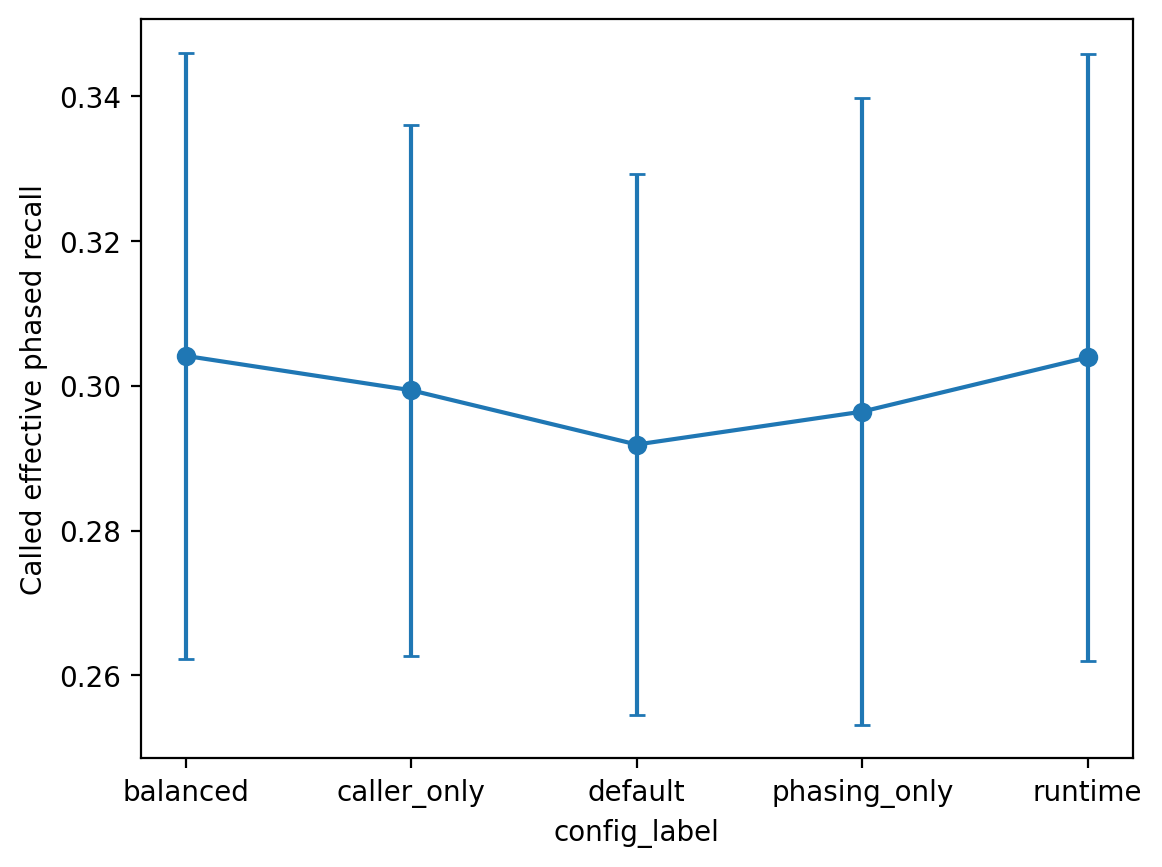
\includegraphics[width=0.82\linewidth]{figures/10_experiments/fig_10_9_8_1_called_effective_phased_recall.png}
\end{center}

\textbf{Figure 10.9.8.1 --- Called effective phased recall across
representative configurations.} The balanced configuration achieves the
highest end-to-end phased recall, while the runtime-biased configuration
performs almost identically. This shows that combining caller-side and
phasing-side tuning yields the strongest practical performance.

\textbf{Figure 10.9.8.2 --- Called shared heterozygous recall across
representative configurations.} Called shared heterozygous recall is
highest for the configurations that use the improved caller threshold,
confirming that part of the overall gain comes from recovering more true
heterozygous sites before phasing.

\textbf{Figure 10.9.8.3 --- Called number of phase sets across
representative configurations.}\\
Phase fragmentation is much lower in the phasing-tuned, balanced, and
runtime configurations than in the default or caller-only
configurations. This shows that phasing-side tuning is the main driver
of improved block continuity.

\textbf{Figure 10.9.8.4 --- Total pipeline runtime across representative
configurations.}\\
Runtime differences between the representative configurations are
modest, but the balanced and runtime-biased settings both remain
competitive while outperforming the default configuration on the main
phasing metrics.

\paragraph{Results summary}\label{results-summary-7}

Means over 5 seeds:

\begin{itemize}
\tightlist
\item
  \textbf{\texttt{default}}

  \begin{itemize}
  \tightlist
  \item
    \texttt{time\_total\_sec}: 3.9338
  \item
    \texttt{call\_precision}: 0.9994
  \item
    \texttt{call\_recall}: 0.5895
  \item
    \texttt{oracle\_effective\_phased\_recall}: 0.8298
  \item
    \texttt{oracle\_num\_phase\_sets}: 6.2
  \item
    \texttt{called\_effective\_phased\_recall}: 0.2919
  \item
    \texttt{called\_shared\_het\_recall}: 0.5098
  \item
    \texttt{called\_phasing\_rate\_shared\_het}: 0.5864
  \item
    \texttt{called\_switch\_error}: 0.0056
  \item
    \texttt{called\_num\_phase\_sets}: 9.6
  \end{itemize}
\item
  \textbf{\texttt{caller\_only}}

  \begin{itemize}
  \tightlist
  \item
    \texttt{time\_total\_sec}: 4.0540
  \item
    \texttt{call\_precision}: 0.9995
  \item
    \texttt{call\_recall}: 0.5970
  \item
    \texttt{oracle\_effective\_phased\_recall}: 0.8298
  \item
    \texttt{oracle\_num\_phase\_sets}: 6.2
  \item
    \texttt{called\_effective\_phased\_recall}: 0.2994
  \item
    \texttt{called\_shared\_het\_recall}: 0.5181
  \item
    \texttt{called\_phasing\_rate\_shared\_het}: 0.5934
  \item
    \texttt{called\_switch\_error}: 0.0077
  \item
    \texttt{called\_num\_phase\_sets}: 9.0
  \end{itemize}
\item
  \textbf{\texttt{phasing\_only}}

  \begin{itemize}
  \tightlist
  \item
    \texttt{time\_total\_sec}: 3.7970
  \item
    \texttt{call\_precision}: 0.9994
  \item
    \texttt{call\_recall}: 0.5895
  \item
    \texttt{oracle\_effective\_phased\_recall}: 0.9402
  \item
    \texttt{oracle\_num\_phase\_sets}: 3.8
  \item
    \texttt{called\_effective\_phased\_recall}: 0.2964
  \item
    \texttt{called\_shared\_het\_recall}: 0.5098
  \item
    \texttt{called\_phasing\_rate\_shared\_het}: 0.6027
  \item
    \texttt{called\_switch\_error}: 0.0007
  \item
    \texttt{called\_num\_phase\_sets}: 6.6
  \end{itemize}
\item
  \textbf{\texttt{balanced}}

  \begin{itemize}
  \tightlist
  \item
    \texttt{time\_total\_sec}: 3.8682
  \item
    \texttt{call\_precision}: 0.9995
  \item
    \texttt{call\_recall}: 0.5970
  \item
    \texttt{oracle\_effective\_phased\_recall}: 0.9402
  \item
    \texttt{oracle\_num\_phase\_sets}: 3.8
  \item
    \texttt{called\_effective\_phased\_recall}: 0.3041
  \item
    \texttt{called\_shared\_het\_recall}: 0.5181
  \item
    \texttt{called\_phasing\_rate\_shared\_het}: 0.6090
  \item
    \texttt{called\_switch\_error}: 0.0007
  \item
    \texttt{called\_num\_phase\_sets}: 6.6
  \end{itemize}
\item
  \textbf{\texttt{runtime}}

  \begin{itemize}
  \tightlist
  \item
    \texttt{time\_total\_sec}: 3.8504
  \item
    \texttt{call\_precision}: 0.9995
  \item
    \texttt{call\_recall}: 0.5970
  \item
    \texttt{oracle\_effective\_phased\_recall}: 0.9348
  \item
    \texttt{oracle\_num\_phase\_sets}: 3.8
  \item
    \texttt{called\_effective\_phased\_recall}: 0.3039
  \item
    \texttt{called\_shared\_het\_recall}: 0.5181
  \item
    \texttt{called\_phasing\_rate\_shared\_het}: 0.6090
  \item
    \texttt{called\_switch\_error}: 0.0022
  \item
    \texttt{called\_num\_phase\_sets}: 6.6
  \end{itemize}
\end{itemize}

\paragraph{Key observations}\label{key-observations-14}

\begin{itemize}
\item
  O1 (The balanced configuration provides the best overall trade-off):
  Among the representative configurations, \texttt{balanced} achieves
  the highest called effective phased recall (\texttt{0.3041}) while
  also maintaining low fragmentation (\texttt{6.6} phase sets), very low
  switch error (\texttt{0.0007}), and lower runtime than the default
  configuration.
\item
  O2 (Default is dominated by the tuned configurations): The default
  configuration is worse than \texttt{balanced} and \texttt{runtime} on
  called effective phased recall, called shared heterozygous recall,
  switch error, and fragmentation, while also not being the fastest
  option. This indicates that the untuned hard-scenario settings are not
  practically competitive.
\item
  O3 (Caller-only and phasing-only tuning recover complementary parts of
  the gain): \texttt{caller\_only} improves overlap-related metrics
  (\texttt{call\_recall}, \texttt{called\_shared\_het\_recall}) but
  leaves fragmentation high, whereas \texttt{phasing\_only} strongly
  improves continuity and oracle phasing metrics but does not recover
  additional called-site overlap. The balanced configuration combines
  both benefits.
\item
  O4 (The runtime-biased configuration is a viable alternative):
  \texttt{runtime} performs almost identically to \texttt{balanced} on
  the main called metrics (\texttt{0.3039} vs \texttt{0.3041} called
  effective phased recall) while using a slightly lower
  \texttt{max\_coverage}. This makes it a reasonable alternative when
  efficiency is prioritized, although \texttt{balanced} remains the
  cleaner general recommendation.
\end{itemize}

\paragraph{Takeaway}\label{takeaway-14}

The frontier comparison shows that the best practical performance comes
from combining moderate caller-side and phasing-side tuning rather than
optimizing either stage in isolation. The balanced configuration is the
preferred general setting because it delivers the highest end-to-end
phased recall together with strong continuity and low switch error. A
slightly more runtime-biased configuration performs almost identically
and may be acceptable when efficiency is prioritized, but the default
configuration is clearly dominated.

\subsubsection{10.9.9 Optimization robustness across
scenarios}\label{optimization-robustness-across-scenarios}

\paragraph{Setup}\label{setup-15}

To test whether the recommended optimized settings generalize beyond the
hard tuning scenario, three representative configurations were compared
across four scenarios:

Configurations compared: - \textbf{\texttt{default}} -
\textbf{\texttt{balanced}} - \textbf{\texttt{runtime}}

Scenarios compared: - \textbf{baseline} - \textbf{dropout} -
\textbf{interaction} - \textbf{hard}

The aim was to determine whether the recommended tuning is broadly
useful or only beneficial in the hard scenario used for parameter
selection.

\paragraph{Figures to include}\label{figures-to-include-15}

\begin{itemize}
\tightlist
\item
  \textbf{Figure 10.9.9.1 --- Called effective phased recall across
  scenarios and representative configurations (heatmap).}
\item
  \textbf{Figure 10.9.9.2 --- Called shared heterozygous recall across
  scenarios and representative configurations.}
\item
  \textbf{Figure 10.9.9.3 --- Called number of phase sets across
  scenarios and representative configurations.}
\item
  \textbf{Figure 10.9.9.4 --- Total pipeline runtime across scenarios
  and representative configurations.}
\end{itemize}

\begin{center}
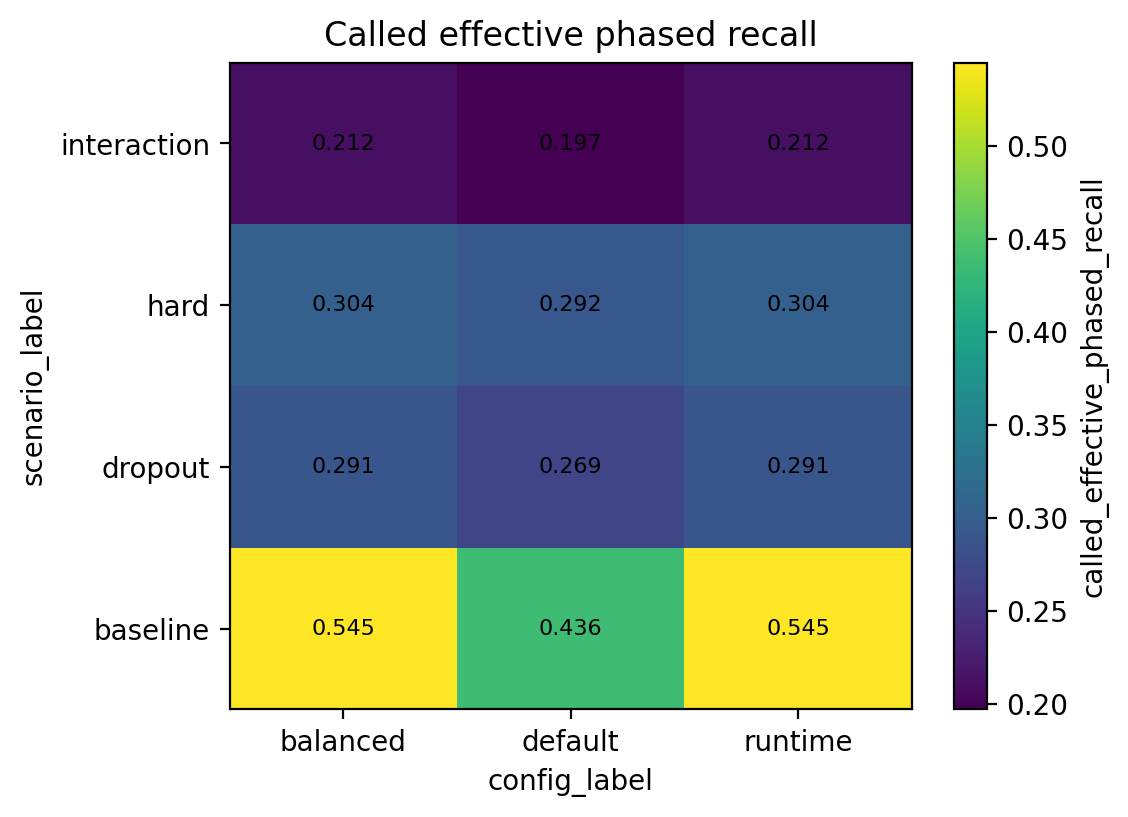
\includegraphics[width=0.88\linewidth]{figures/10_experiments/fig_10_9_9_1_called_effective_phased_recall_heatmap.png}
\end{center}

\textbf{Figure 10.9.9.1 --- Called effective phased recall across
scenarios and representative configurations.} Across all tested
scenarios, the balanced and runtime configurations achieve higher
end-to-end phased recall than the default configuration, showing that
the selected tuning generalizes beyond the hard optimization scenario.

\textbf{Figure 10.9.9.2 --- Called shared heterozygous recall across
scenarios and representative configurations.}\\
The tuned configurations consistently improve called shared heterozygous
recall, indicating that part of the transferable gain comes from
recovering more true heterozygous sites across multiple scenarios.

\textbf{Figure 10.9.9.3 --- Called number of phase sets across scenarios
and representative configurations.}\\
The balanced and runtime configurations reduce phase fragmentation
relative to the default configuration in all tested scenarios, showing
that the tuning also improves block continuity rather than only site
recovery.

\textbf{Figure 10.9.9.4 --- Total pipeline runtime across scenarios and
representative configurations.}\\
Runtime remains competitive for the tuned configurations across
scenarios, and the runtime-biased variant offers nearly identical
accuracy with similar or slightly improved efficiency.

\paragraph{Results summary}\label{results-summary-8}

Means over 5 seeds:

\begin{itemize}
\tightlist
\item
  \textbf{Baseline}

  \begin{itemize}
  \tightlist
  \item
    \texttt{default}:
    \texttt{called\_effective\_phased\_recall\ =\ 0.4364},
    \texttt{called\_shared\_het\_recall\ =\ 0.5902},
    \texttt{called\_num\_phase\_sets\ =\ 3.4},
    \texttt{time\_total\_sec\ =\ 2.9850}
  \item
    \texttt{balanced}: \texttt{0.5448}, \texttt{0.6097}, \texttt{1.4},
    \texttt{3.0223}
  \item
    \texttt{runtime}: \texttt{0.5448}, \texttt{0.6097}, \texttt{1.4},
    \texttt{2.9596}
  \end{itemize}
\item
  \textbf{Dropout}

  \begin{itemize}
  \tightlist
  \item
    \texttt{default}: \texttt{0.2694}, \texttt{0.5292}, \texttt{6.2},
    \texttt{2.9768}
  \item
    \texttt{balanced}: \texttt{0.2908}, \texttt{0.5420}, \texttt{4.2},
    \texttt{2.9362}
  \item
    \texttt{runtime}: \texttt{0.2908}, \texttt{0.5420}, \texttt{4.2},
    \texttt{2.9391}
  \end{itemize}
\item
  \textbf{Interaction}

  \begin{itemize}
  \tightlist
  \item
    \texttt{default}: \texttt{0.1972}, \texttt{0.5014}, \texttt{6.2},
    \texttt{3.0043}
  \item
    \texttt{balanced}: \texttt{0.2118}, \texttt{0.5094}, \texttt{5.4},
    \texttt{2.8789}
  \item
    \texttt{runtime}: \texttt{0.2118}, \texttt{0.5094}, \texttt{5.4},
    \texttt{2.9750}
  \end{itemize}
\item
  \textbf{Hard}

  \begin{itemize}
  \tightlist
  \item
    \texttt{default}: \texttt{0.2919}, \texttt{0.5098}, \texttt{9.6},
    \texttt{4.3644}
  \item
    \texttt{balanced}: \texttt{0.3041}, \texttt{0.5181}, \texttt{6.6},
    \texttt{4.2497}
  \item
    \texttt{runtime}: \texttt{0.3039}, \texttt{0.5181}, \texttt{6.6},
    \texttt{4.3050}
  \end{itemize}
\end{itemize}

\paragraph{Key observations}\label{key-observations-15}

\begin{itemize}
\item
  O1 (The tuned configurations generalize across scenarios): In all four
  scenarios, both \texttt{balanced} and \texttt{runtime} outperform
  \texttt{default} on called effective phased recall and called shared
  heterozygous recall. This shows that the tuned settings are not
  overfit to the hard scenario alone.
\item
  O2 (The balanced configuration is the safest general recommendation):
  \texttt{balanced} is never worse than \texttt{default} and is either
  best or tied for best on the main called metrics across all scenarios.
  This supports its use as the default recommended configuration.
\item
  O3 (The runtime-biased configuration is highly competitive):
  \texttt{runtime} is effectively identical to \texttt{balanced} on the
  main called metrics in this sweep and remains competitive on runtime.
  This makes it a reasonable alternative when efficiency is prioritized.
\item
  O4 (The gains transfer to both easy and hard cases): The tuned
  configurations improve performance not only in the hard scenario, but
  also in the baseline, dropout, and interaction scenarios. This
  indicates that the optimization is robust across qualitatively
  different data conditions.
\end{itemize}

\paragraph{Takeaway}\label{takeaway-15}

The recommended tuned settings are robust across the representative
scenarios tested in this study. The balanced configuration is the
cleanest general recommendation because it consistently improves
end-to-end phased recall and reduces fragmentation relative to the
default. A runtime-biased alternative performs almost identically and
may be preferred when efficiency is prioritized.

\subsubsection{\texorpdfstring{10.9.10 Sweep H: caller
\texttt{call\_min\_mapq}
rule-out}{10.9.10 Sweep H: caller call\_min\_mapq rule-out}}\label{sweep-h-caller-call_min_mapq-rule-out}

\paragraph{Setup}\label{setup-16}

A final small rule-out sweep was conducted to test whether caller
mapping-quality filtering provides meaningful optimization headroom once
the other recommended settings are fixed.

\begin{itemize}
\tightlist
\item
  Varied:

  \begin{itemize}
  \tightlist
  \item
    \texttt{call\_min\_mapq\ ∈\ \{0,\ 10,\ 20\}}
  \end{itemize}
\item
  Fixed:

  \begin{itemize}
  \tightlist
  \item
    \texttt{call\_min\_baseq\ =\ 10}
  \item
    \texttt{max\_coverage\ =\ 8}
  \item
    \texttt{min\_mapq\ =\ 20}
  \item
    \texttt{min\_baseq\ =\ 10}
  \item
    hard-scenario stressors unchanged
  \end{itemize}
\end{itemize}

\paragraph{Figures to include}\label{figures-to-include-16}

\begin{itemize}
\tightlist
\item
  \textbf{Figure 10.9.10.1 --- Called effective phased recall vs
  \texttt{call\_min\_mapq}.}
\item
  \textbf{Figure 10.9.10.2 --- Calling recall vs
  \texttt{call\_min\_mapq}.}
\item
  \textbf{Figure 10.9.10.3 --- Called shared heterozygous recall vs
  \texttt{call\_min\_mapq}.}
\item
  \textbf{Figure 10.9.10.4 --- Call precision vs
  \texttt{call\_min\_mapq}.}
\end{itemize}

\textbf{Figure 10.9.10.1 --- Called effective phased recall vs
\texttt{call\_min\_mapq}.}\\
Called effective phased recall changes only slightly across the caller
mapping-quality sweep, indicating that \texttt{call\_min\_mapq} is not a
strong optimization lever under the current hard scenario.

\textbf{Figure 10.9.10.2 --- Calling recall vs
\texttt{call\_min\_mapq}.}\\
Calling recall remains essentially unchanged across the caller
mapping-quality sweep, showing that mapQ filtering has little influence
on variant recovery in this setup.

\textbf{Figure 10.9.10.3 --- Called shared heterozygous recall vs
\texttt{call\_min\_mapq}.}\\
Called shared heterozygous recall is nearly flat across the caller
mapping-quality sweep, confirming that caller mapQ does not materially
alter the overlap of useful true heterozygous sites.

\textbf{Figure 10.9.10.4 --- Call precision vs
\texttt{call\_min\_mapq}.}\\
Call precision remains extremely high across all caller mapping-quality
settings, indicating that stricter mapQ filtering does not provide a
meaningful precision advantage in this pipeline.

\paragraph{Results summary}\label{results-summary-9}

Means over 5 seeds:

\begin{itemize}
\tightlist
\item
  \texttt{call\_min\_mapq\ =\ 0}

  \begin{itemize}
  \tightlist
  \item
    \texttt{call\_precision\ =\ 0.9995}
  \item
    \texttt{call\_recall\ =\ 0.5962}
  \item
    \texttt{called\_shared\_het\_recall\ =\ 0.5171}
  \item
    \texttt{called\_effective\_phased\_recall\ =\ 0.3155}
  \item
    \texttt{called\_phasing\_rate\_shared\_het\ =\ 0.6102}
  \item
    \texttt{called\_phase\_accuracy\ =\ 1.0000}
  \item
    \texttt{called\_switch\_error\ =\ 0.0000}
  \item
    \texttt{time\_total\_sec\ =\ 4.1980}
  \end{itemize}
\item
  \texttt{call\_min\_mapq\ =\ 10}

  \begin{itemize}
  \tightlist
  \item
    \texttt{call\_precision\ =\ 0.9995}
  \item
    \texttt{call\_recall\ =\ 0.5970}
  \item
    \texttt{called\_shared\_het\_recall\ =\ 0.5181}
  \item
    \texttt{called\_effective\_phased\_recall\ =\ 0.3157}
  \item
    \texttt{called\_phasing\_rate\_shared\_het\ =\ 0.6094}
  \item
    \texttt{called\_phase\_accuracy\ =\ 1.0000}
  \item
    \texttt{called\_switch\_error\ =\ 0.0000}
  \item
    \texttt{time\_total\_sec\ =\ 4.1432}
  \end{itemize}
\item
  \texttt{call\_min\_mapq\ =\ 20}

  \begin{itemize}
  \tightlist
  \item
    \texttt{call\_precision\ =\ 0.9995}
  \item
    \texttt{call\_recall\ =\ 0.5970}
  \item
    \texttt{called\_shared\_het\_recall\ =\ 0.5181}
  \item
    \texttt{called\_effective\_phased\_recall\ =\ 0.3041}
  \item
    \texttt{called\_phasing\_rate\_shared\_het\ =\ 0.6090}
  \item
    \texttt{called\_phase\_accuracy\ =\ 0.9622}
  \item
    \texttt{called\_switch\_error\ =\ 0.0007}
  \item
    \texttt{time\_total\_sec\ =\ 4.1246}
  \end{itemize}
\end{itemize}

\paragraph{Key observations}\label{key-observations-16}

\begin{itemize}
\item
  O1 (Caller mapping-quality filtering has little effect on overlap
  recovery): Calling recall and called shared heterozygous recall remain
  essentially unchanged across
  \texttt{call\_min\_mapq\ ∈\ \{0,\ 10,\ 20\}}. This indicates that
  caller mapping-quality filtering does not materially alter the amount
  of useful variant evidence reaching the phasing stage.
\item
  O2 (The optimization signal is much weaker than for caller
  base-quality): In contrast to the earlier caller base-quality sweep,
  changing \texttt{call\_min\_mapq} produces only very small differences
  in the main called metrics. This shows that caller mapping-quality is
  not a strong optimization lever in the current pipeline.
\item
  O3 (No compelling benefit is obtained from stricter caller mapQ
  filtering): Although \texttt{call\_min\_mapq\ =\ 20} shows a slight
  reduction in called effective phased recall, the effect is small and
  not accompanied by meaningful changes in call precision or shared-site
  recall. This suggests that aggressive caller mapQ filtering provides
  no practical advantage here.
\end{itemize}

\paragraph{Takeaway}\label{takeaway-16}

Caller mapping-quality filtering does not provide meaningful
optimization headroom under the current hard scenario. Unlike caller
base-quality, which showed a clear and useful tuning signal,
\texttt{call\_min\_mapq} has only weak effects on the main end-to-end
phasing metrics. This supports treating caller mapQ as a low-priority or
effectively negligible optimization knob in this pipeline.

\subsubsection{10.9.11 DP-scaling under hard
conditions}\label{dp-scaling-under-hard-conditions}

\paragraph{Aim}\label{aim-8}

Assess how the downstream phasing problem scales with increasing SNP
density under the composite hard scenario, and determine whether the
tuned configuration changes the runtime growth of the solve stage.

\paragraph{Setup}\label{setup-17}

A small scaling study was conducted under the fixed hard scenario,
varying only the number of SNPs:

\begin{itemize}
\tightlist
\item
  \texttt{num\_snps\ ∈\ \{400,\ 800,\ 1200,\ 1600\}}
\end{itemize}

Two configurations were compared: - \textbf{\texttt{default}} -
\texttt{call\_min\_baseq\ =\ 15} - \texttt{max\_coverage\ =\ 15} -
\texttt{min\_baseq\ =\ 20} - \textbf{\texttt{balanced}} -
\texttt{call\_min\_baseq\ =\ 10} - \texttt{max\_coverage\ =\ 8} -
\texttt{min\_baseq\ =\ 10}

All other hard-scenario stressors were kept fixed.

\paragraph{Figures to include}\label{figures-to-include-17}

\begin{itemize}
\tightlist
\item
  \textbf{Figure 10.9.11.1 --- Called solve time vs SNP count under
  default and optimized configurations.}
\item
  \textbf{Figure 10.9.11.2 --- Oracle solve time vs SNP count under
  default and optimized configurations.}
\item
  \textbf{Figure 10.9.11.3 --- Called effective phased recall vs SNP
  count under default and optimized configurations.}
\item
  \textbf{Figure 10.9.11.4 --- Called number of phase sets vs SNP count
  under default and optimized configurations.}
\end{itemize}

\begin{center}
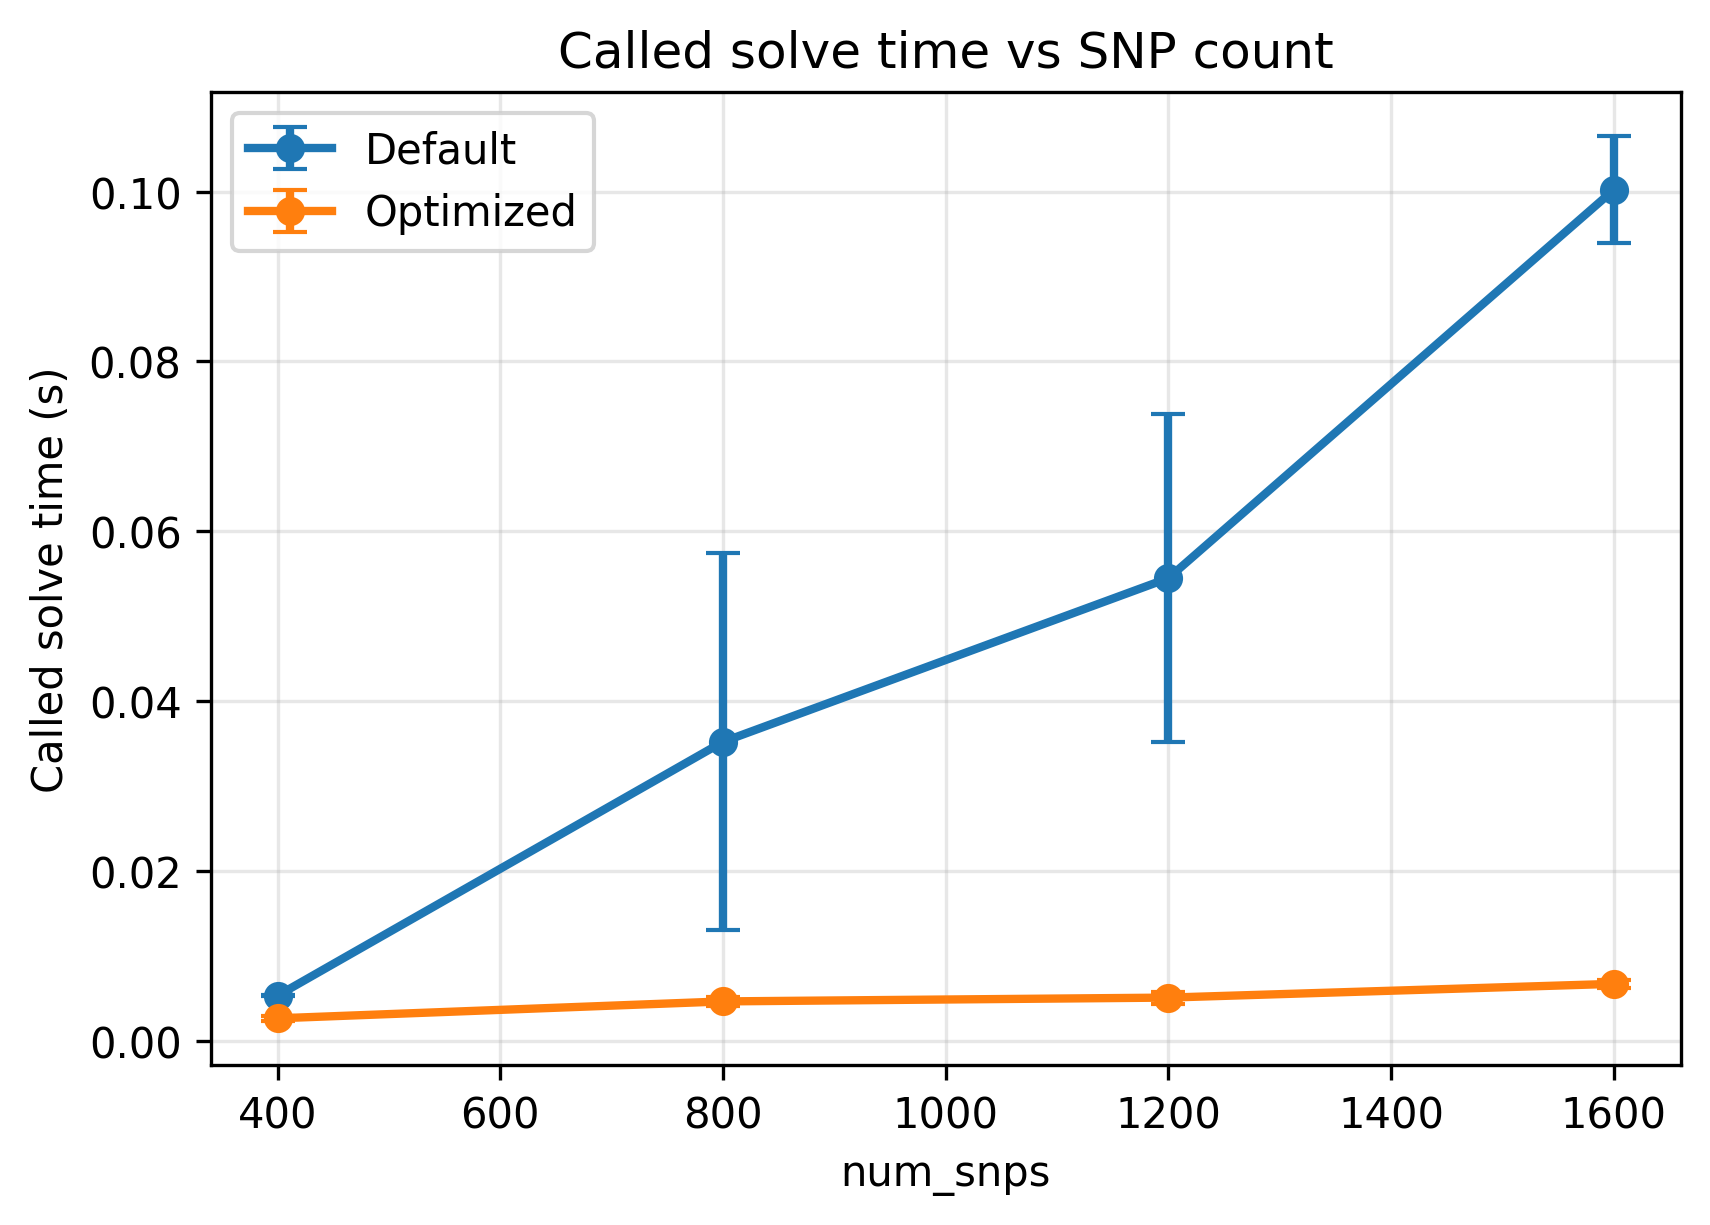
\includegraphics[width=0.82\linewidth]{figures/10_experiments/fig_10_9_11_1_called_time_solve_sec.png}
\end{center}

\textbf{Figure 10.9.11.1 --- Called solve time vs SNP count under
default and optimized configurations.} Called solve time increases with
SNP density under both configurations, but grows much more steeply under
the default setting. This shows that the tuned configuration makes the
residual phasing problem easier to solve as variant density increases.

\textbf{Figure 10.9.11.2 --- Oracle solve time vs SNP count under
default and optimized configurations.}\\
Oracle solve time also increases with SNP density, confirming that the
solver becomes more expensive as the phasing-only problem grows. The
optimized configuration remains substantially faster, indicating that
its benefit is not solely due to changes in the called callset.

\textbf{Figure 10.9.11.3 --- Called effective phased recall vs SNP count
under default and optimized configurations.}\\
Across the scaling range, the optimized configuration maintains slightly
higher end-to-end phased recall than the default configuration, showing
that its runtime benefit is not obtained by sacrificing phasing quality.

\textbf{Figure 10.9.11.4 --- Called number of phase sets vs SNP count
under default and optimized configurations.}\\
The optimized configuration generally produces fewer phase sets than the
default configuration as SNP density increases, indicating better
phase-block continuity and a less fragmented residual phasing problem.

\paragraph{Results summary}\label{results-summary-10}

Means over 3 seeds:

\begin{itemize}
\tightlist
\item
  \textbf{optimized}

  \begin{itemize}
  \tightlist
  \item
    \texttt{called\_time\_solve\_sec}:
    \texttt{0.0026\ →\ 0.0046\ →\ 0.0051\ →\ 0.0067}
  \item
    \texttt{oracle\_time\_solve\_sec}:
    \texttt{0.0044\ →\ 0.0066\ →\ 0.0091\ →\ 0.0114}
  \item
    \texttt{called\_effective\_phased\_recall}:
    \texttt{0.3071\ →\ 0.3705\ →\ 0.3295\ →\ 0.3280}
  \item
    \texttt{called\_num\_phase\_sets}:
    \texttt{6.0\ →\ 5.7\ →\ 7.3\ →\ 6.3}
  \end{itemize}
\item
  \textbf{Default}

  \begin{itemize}
  \tightlist
  \item
    \texttt{called\_time\_solve\_sec}:
    \texttt{0.0053\ →\ 0.0352\ →\ 0.0545\ →\ 0.1002}
  \item
    \texttt{oracle\_time\_solve\_sec}:
    \texttt{0.0114\ →\ 0.0533\ →\ 0.0863\ →\ 0.1407}
  \item
    \texttt{called\_effective\_phased\_recall}:
    \texttt{0.2935\ →\ 0.3539\ →\ 0.3164\ →\ 0.3141}
  \item
    \texttt{called\_num\_phase\_sets}:
    \texttt{8.3\ →\ 10.7\ →\ 10.0\ →\ 7.7}
  \end{itemize}
\end{itemize}

\paragraph{Key observations}\label{key-observations-17}

\begin{itemize}
\item
  O1 (Solve time increases with SNP density): In both oracle and called
  regimes, solve time increases as \texttt{num\_snps} increases from 400
  to 1600, showing that the downstream phasing problem becomes more
  expensive as variant density rises.
\item
  O2 (The optimized configuration scales much better than default): The
  growth in solve time is much steeper under the default configuration
  than under the optimized configuration. At
  \texttt{num\_snps\ =\ 1600}, default solve time is substantially
  higher than optimized in both oracle and called regimes, indicating
  that the tuned settings make the residual phasing problem easier to
  solve.
\item
  O3 (optimized remains better on phasing continuity as the problem
  grows): Across the scaling range, the optimized configuration
  generally maintains fewer phase sets and slightly better phased recall
  than the default configuration. This suggests that the tuning improves
  not only final phasing output but also the structure of the instance
  presented to the solver.
\item
  O4 (Solve time still does not dominate total runtime end-to-end):
  Although solve time grows with SNP density, total phasing runtime
  remains dominated by preprocessing/readset construction in the current
  research pipeline. Therefore, the main value of this result is
  algorithmic interpretation rather than end-to-end runtime engineering.
\end{itemize}

\paragraph{Takeaway}\label{takeaway-17}

The DP-scaling study shows that increasing SNP density makes the phasing
solve stage progressively more expensive, but also that the optimized
tuned configuration scales substantially better than the default
configuration. This suggests that practical tuning can improve not only
phased output quality but also the difficulty of the residual wMEC-style
problem faced by the solver.

\subsubsection{Overall takeaway}\label{overall-takeaway}

Under the current hard scenario, optimization headroom exists but is
uneven across knobs. WhatsHap-side tuning provides only limited gains:
increasing \texttt{max\_coverage} does not help, and the main useful
phasing-side adjustment is to avoid overly strict \texttt{min\_baseq}
filtering. In contrast, caller-side tuning is more impactful: lowering
\texttt{call\_min\_baseq} from 20 to a moderate value such as 10
improves variant recovery, shared heterozygous overlap, and end-to-end
phased recall without materially reducing precision. Taken together,
these results indicate that practical optimization in this pipeline is
not purely a WhatsHap parameter problem; meaningful gains are more
likely to come from a combination of permissive phasing evidence
retention and improved upstream variant recovery.

\begin{center}\rule{0.5\linewidth}{0.5pt}\end{center}

\subsection{10.10 Summary of results (cross-experiment
synthesis)}\label{summary-of-results-cross-experiment-synthesis}

\subsubsection{10.10.1 Attribution summary (oracle vs
called)}\label{attribution-summary-oracle-vs-called}

Taken together, the oracle-vs-called comparison provides a consistent
attribution picture across the stress studies.

\begin{itemize}
\item
  \textbf{Duplications:} primarily a \textbf{called-regime
  phasing/evidence-quality stressor}, rather than a strong
  caller-limited bottleneck. Calling recall remains nearly unchanged
  across duplication levels, and oracle effective phased recall remains
  high and stable. The main degradation appears only at the strongest
  duplication level, where called phasing completeness and phase
  accuracy worsen without a corresponding drop in shared-site recall.
  This indicates that duplicated regions mainly weaken the consistency
  of phasing evidence on surviving called sites.
\item
  \textbf{Coverage dropout:} primarily a \textbf{fragmentation-dominated
  stressor}, becoming \textbf{mixed} at high severity. Oracle phase-set
  counts increase strongly with dropout fraction and oracle effective
  phased recall declines, showing that dropout directly breaks read
  connectivity even when correct sites are supplied. In the called
  regime, performance degrades more strongly still, and at severe
  dropout both shared-site recall and phasing completeness collapse.
  This makes dropout the clearest example of a connectivity bottleneck
  that later becomes both a calling and phasing bottleneck.
\item
  \textbf{Correlated error bursts:} a \textbf{weak and somewhat noisy
  called-regime correctness stressor} under the current
  parameterization. Oracle metrics remain stable, calling recall is
  broadly unchanged, and the main visible effect is a dip in
  called-regime phase accuracy and switch stability at intermediate
  burst probability. Because the response is non-monotonic, this
  stressor should be interpreted cautiously and does not currently
  provide a strong optimization signal.
\item
  \textbf{Read length model:} a \textbf{mixed continuity/overlap
  trade-off} rather than a clear stressor or optimization knob. The
  lognormal model improves calling recall, shared-site recall, and
  phase-block continuity, but these gains are largely offset by slightly
  worse called-regime phasing correctness. This shows that better
  connectivity alone does not guarantee a strong end-to-end gain.
\item
  \textbf{Truth indels with SNP-only policy:} primarily a
  \textbf{methodology-validity result}, not a performance stressor.
  Oracle SNP-phasing metrics remain stable and called SNP-level metrics
  stay within a comparable range across indel settings, indicating that
  \texttt{phase\_snps\_only} and \texttt{eval\_snps\_only} successfully
  preserve interpretable SNP phasing evaluation even when truth indels
  are present.
\item
  \textbf{Duplication × dropout interaction:} a \textbf{mixed compounded
  weakness}, strongest in the called regime. Dropout remains the main
  source of fragmentation, but duplication further worsens both
  called-site overlap and phasing completeness on surviving sites. This
  interaction shows that realistic end-to-end failure modes arise most
  clearly when ambiguous mapping and low-coverage gaps are combined.
\end{itemize}

Overall, the attribution pattern is consistent: whenever oracle
performance remains strong but called performance degrades, the dominant
bottleneck lies in the overlap and quality of called heterozygous sites.
When oracle performance also degrades, the stressor is directly harming
phase-block connectivity or phasing completeness.

\subsubsection{10.10.2 Most impactful
stressors}\label{most-impactful-stressors}

Across the single-knob and interaction studies, the realism knobs differ
substantially in practical impact.

\begin{itemize}
\item
  \textbf{Most impactful overall:} \textbf{coverage dropout}. It
  produces the clearest and strongest reduction in called effective
  phased recall, strongly increases phase fragmentation, and eventually
  also reduces calling recall. It is the most important isolated
  stressor in this study.
\item
  \textbf{Most impactful compounded weakness:} \textbf{duplication ×
  dropout interaction}. While duplication alone is relatively mild, its
  combination with dropout creates a substantially worse end-to-end
  condition than either stressor alone, especially in the called regime.
  This reveals a realistic mixed failure mode involving both reduced
  callable overlap and weaker phasing connectivity.
\item
  \textbf{Moderate impact:} \textbf{read length model} and
  \textbf{strong duplication}. The read length model changes continuity
  and overlap in opposite directions, while strong duplication mainly
  affects called-regime phasing quality at the highest severity.
\item
  \textbf{Weak / noisy impact:} \textbf{correlated error bursts}. Under
  the current parameterization, bursts do not produce a strong monotonic
  degradation trend and therefore are less informative as a practical
  optimization target.
\item
  \textbf{Methodological rather than stress-inducing:} \textbf{truth
  indels under SNP-only policy}. Their main value is to validate that
  the evaluation remains interpretable under indel-containing truth
  sets.
\end{itemize}

If stressors are ranked by effect on the main end-to-end metric
(\texttt{called\_effective\_phased\_recall}), the most important
findings are:\\
1. \textbf{dropout},\\
2. \textbf{duplication × dropout interaction},\\
3. \textbf{strong duplication / read-length trade-off effects},\\
4. \textbf{bursts (weak/noisy)},\\
with the indel study serving primarily as an evaluation-robustness check
rather than a degradation study.

\subsubsection{10.10.3 Optimization summary}\label{optimization-summary}

Optimization sweeps under the composite hard scenario showed that
optimization headroom exists, but is uneven across knobs.

A small runtime breakdown of the called phasing stage was also examined
for representative configurations under the hard scenario:

{\def\LTcaptype{none} % do not increment counter
\begin{longtable}[]{@{}
  >{\raggedright\arraybackslash}p{(\linewidth - 8\tabcolsep) * \real{0.1579}}
  >{\raggedleft\arraybackslash}p{(\linewidth - 8\tabcolsep) * \real{0.2105}}
  >{\raggedleft\arraybackslash}p{(\linewidth - 8\tabcolsep) * \real{0.2105}}
  >{\raggedleft\arraybackslash}p{(\linewidth - 8\tabcolsep) * \real{0.2105}}
  >{\raggedleft\arraybackslash}p{(\linewidth - 8\tabcolsep) * \real{0.2105}}@{}}
\toprule\noalign{}
\begin{minipage}[b]{\linewidth}\raggedright
Configuration
\end{minipage} & \begin{minipage}[b]{\linewidth}\raggedleft
Build ReadSet (s)
\end{minipage} & \begin{minipage}[b]{\linewidth}\raggedleft
Read Selection (s)
\end{minipage} & \begin{minipage}[b]{\linewidth}\raggedleft
Solve (s)
\end{minipage} & \begin{minipage}[b]{\linewidth}\raggedleft
Called Phasing Total (s)
\end{minipage} \\
\midrule\noalign{}
\endhead
\bottomrule\noalign{}
\endlastfoot
Optimized & 0.3679 & 0.0061 & 0.0056 & 0.3854 \\
Default & 0.3734 & 0.0023 & 0.0610 & 0.4433 \\
Speed-oriented & 0.3685 & 0.0050 & 0.0030 & 0.3827 \\
\end{longtable}
}

This runtime breakdown shows that, in the current research pipeline, the
largest share of called phasing runtime is spent in readset
construction, while read selection and the downstream solve stage
contribute smaller but configuration-dependent fractions. In particular,
the default configuration has a noticeably larger solve-stage cost than
the tuned configurations, whereas the optimized and speed-oriented
settings are dominated even more strongly by readset construction. This
result should be interpreted cautiously, because the present study uses
a custom adaptor to support oracle/called benchmarking and unified
reporting rather than the standard production-facing WhatsHap front-end.
Nevertheless, it suggests that evidence extraction can be a significant
practical cost in WhatsHap-based phasing workflows, and that the tuned
configurations improve runtime mainly through a better overall phasing
setup rather than through a large reduction in the core solve stage
alone.

The main optimization findings are:

\begin{itemize}
\item
  \textbf{Useful caller-side knob:} \texttt{call\_min\_baseq}. Lowering
  the caller base-quality threshold from 20 to a moderate value such as
  10 substantially improves calling recall, shared heterozygous overlap,
  and end-to-end phased recall without materially harming precision.
  This is the strongest optimization signal found in the study.
\item
  \textbf{Useful phasing-side knob:} \texttt{min\_baseq}, but mainly as
  a \textbf{rule-out of overly strict filtering}. Phasing performance is
  stable for \texttt{min\_baseq\ =\ 0–15}, but degrades at \texttt{20},
  indicating that strict phasing base-quality filtering discards too
  much informative evidence. A moderate setting such as
  \texttt{min\_baseq\ =\ 10} is the cleanest practical recommendation.
\item
  \textbf{Useful runtime knob:} \texttt{max\_coverage}. Increasing
  \texttt{max\_coverage} beyond 8--10 does not improve phasing
  performance, while lower values such as 8 preserve full performance
  with lower runtime. This makes \texttt{max\_coverage\ =\ 8} a
  practical efficiency setting.
\item
  \textbf{Weak / negligible knobs:} caller \texttt{call\_min\_mapq},
  phasing \texttt{min\_mapq}, and high \texttt{max\_coverage} values
  above the plateau. These do not provide meaningful practical gains
  under the tested hard scenario.
\item
  \textbf{Robustness of tuning:} the tuned configurations generalize
  across baseline, dropout, interaction, and hard scenarios. In all
  tested cases, the balanced tuned configuration improves called
  effective phased recall and reduces fragmentation relative to default,
  while a runtime-biased configuration performs almost identically and
  remains a viable alternative when efficiency is prioritized.
\item
  \textbf{Algorithm-facing scaling result:} increasing SNP density makes
  the solve stage more expensive, but the balanced tuned configuration
  scales much better than the default configuration. This suggests that
  practical tuning not only improves phased output quality, but also
  reduces the difficulty of the residual wMEC-style problem faced by the
  solver.
\end{itemize}

Based on the optimization sweeps, the recommended practical settings for
this pipeline are:

\begin{itemize}
\tightlist
\item
  \textbf{Recommended \texttt{max\_coverage}:} \texttt{8}\\
\item
  \textbf{Recommended phasing thresholds:} \texttt{min\_mapq\ =\ 20},
  \texttt{min\_baseq\ =\ 10}\\
\item
  \textbf{Recommended calling thresholds:}
  \texttt{call\_min\_mapq\ =\ 20} (or leave at default, as the effect is
  negligible), \texttt{call\_min\_baseq\ =\ 10}
\end{itemize}

A slightly more runtime-biased alternative
(\texttt{max\_coverage\ =\ 6}, with the same caller/phasing quality
thresholds) performs almost identically on the main accuracy metrics and
may be acceptable when efficiency is prioritized.

Future work could compare the custom adaptor against the standard
WhatsHap front-end directly, or optimize the adaptor separately if
pipeline-level runtime becomes a primary objective.

\end{document}
